\section{Eksperimentalna evaluacija i diskusija rezultata}
\label{chap:eksperimenti}
Nakon definiranja teorijskih osnova i implementacije modela, ovo poglavlje posvećeno je empirijskoj validaciji i analizi. Detaljno se opisuje eksperimentalni postav, provedba dvo-faznog istraživanja, te se provodi dubinska analiza i interpretacija dobivenih rezultata. Cilj je kvantificirati performanse predloženih modela i donijeti utemeljene zaključke o njihovoj primjenjivosti.

\subsection{Postavke okruženja i testni podaci}
Svi eksperimenti provedeni su u programskom okruženju \textbf{Python (verzija 3.x)} na standardnom osobnom računalu. Kako bi se osigurala ponovljivost i kontrolirani uvjeti, za potrebe istraživanja generiran je sintetički skup podataka koji oponaša realističan projektni portfelj.  Generiranje podataka je parametrizirano kako bi se mogli stvoriti problemi različite složenosti (broj aktivnosti od 10 do 100). Za svaku aktivnost, vrijednosti troška, ROI-a i trotočkovne procjene trajanja generirane su nasumično unutar realističnih raspona: \textbf{Trošak (\texttt{cost}):} slučajna cjelobrojna vrijednost između 50 i 200, \textbf{ROI (\texttt{roi}):} slučajna decimalna vrijednost između 1.0 i 3.0, i \textbf{Procjene trajanja:} optimistično (između 5 i 10 dana), najvjerojatnije (između 10 i 20 dana) i pesimistično (između 20 i 40 dana).
Ukupni raspoloživi budžet za portfelj (\texttt{BUDGET}) bio je skaliran u skladu sa složenošću problema kako bi se održala slična razina restriktivnosti.

\subsection{Eksperimentalni dizajn}
Kako bi se osigurala metodološka ispravnost i izbjegli proizvoljni zaključci, istraživanje je provedeno kroz dvo-fazni eksperimentalni proces:
\begin{itemize}
    \item \textbf{Faza 1: Analiza i kalibracija genetskog algoritma.} U prvoj fazi provedena je detaljna ablacijska studija kako bi se utvrdilo koji parametri genetskog algoritma daju najkvalitetnija i najstabilnija rješenja za reprezentativni tip problema (50 aktivnosti). Cilj je bio pronaći ``šampionsku'' konfiguraciju GA.
    \item \textbf{Faza 2: Usporedna analiza optimizacijskih modela.} U drugoj fazi, ``šampionska'' konfiguracija GA, dobivena u prvoj fazi, korištena je kao osnova za provođenje konačne usporedbe triju različitih optimizacijskih scenarija i evaluaciju istraživačkih hipoteza: \textbf{H1 (Skalabilnost), H2 (Kompromis) i H3 (Utjecaj Ograničenja)} rada na problemima različite skale i restriktivnosti.
\end{itemize}

\subsubsection{Istraživačke hipoteze}
Na temelju teorijske podloge i postavljenih istraživačkih pitanja iz Uvoda, definirane su sljedeće tri glavne hipoteze koje su vođene ovim istraživanjem i  predstavljaju temelj za analizu i interpretaciju eksperimentalnih rezultata:

\begin{description}

\item \textbf{H1 (Hipoteza o Skalabilnosti):} ``Povećanjem složenosti problema (broja aktivnosti), performanse modela temeljenog na nasumičnoj pretrazi (\texttt{Random Search}) će se značajno smanjiti u usporedbi s modelima temeljenim na genetskim algoritmima.''
Ova hipoteza testira temeljnu prednost inteligentnih metaheuristika. Svrha je dokazati da se, u problemskom prostoru koji eksponencijalno raste s brojem projekata, slijepa, nasumična pretraga brzo gubi u ``astronomski velikom'' prostoru rješenja. S druge strane, genetski algoritmi, s mehanizmima kao što su križanje i mutacija, inteligentno istražuju prostor, usmjeravajući se prema obećavajućim područjima. Ova hipoteza predviđa da će se razlika u performansama između ove dvije metodologije drastično povećati s porastom složenosti problema, čime će se potvrditi nužnost primjene naprednijih metoda.

\item \textbf{H2 (Hipoteza o Kompromisu):} ``Hibridni `GA+MC` model će, za razliku od klasičnog `GA (samo ROI)` modela, uspješno identificirati rješenja koja predstavljaju superioran kompromis između profitabilnosti (\texttt{ROI}) i rizika (trajanje projekta), posebno na problemima veće složenosti.''

Ova hipoteza je srž cijelog rada i istražuje višeciljnu prirodu problema. Dok klasični \texttt{GA} model vidi samo jednu dimenziju (profit), hibridni model, integracijom Monte Carlo simulacije, ``vidi'' i drugu dimenziju (rizik trajanja). Hipoteza predviđa da ova sposobnost istovremene optimizacije dva suprotstavljena cilja neće rezultirati samo jednim rješenjem, već cijelim skupom ne-dominiranih rješenja poznatim kao Pareto front. Očekuje se da će taj skup rješenja pružiti neprocjenjivu stratešku vrijednost, omogućujući menadžeru da kvantificira i odabere optimalan kompromis između maksimizacije profita i minimizacije rizika.

\item \textbf{H3 (Hipoteza o Utjecaju Ograničenja):} ``Restriktivnost problema, specifično kroz promjenu raspoloživog budžeta, značajno utječe na performanse i stabilnost optimizacijskih modela, pri čemu se očekuje da će ekstremna ograničenja predstavljati najveći izazov za najsloženije modele.''

Ova hipoteza testira robusnost modela u nerealističnim, ali izazovnim uvjetima. Umjesto jednostavnog zaključka da je složeniji model uvijek bolji, ova hipoteza predviđa paradoksalan nalaz. Očekuje se da će hibridni, više-kriterijski model, koji briljira u ``otvorenom'' prostoru rješenja, pokazati neočekivanu krhkost kada se prostor rješenja drastično suzi ekstremno niskim budžetom. S druge strane, jednostavniji model fokusiran na jedan cilj (\texttt{ROI}) mogao bi se pokazati robusnijim i stabilnijim u takvim uvjetima. Ova hipoteza naglašava da je odabir najprikladnijeg alata kontekstualan i ovisi o prirodi problema.
\end{description}

\subsection{Eksperiment 1: Analiza parametara i kalibracija genetskog algoritma}

Prvi eksperiment imao je za cilj empirijski provjeriti utjecaj osnovnih genetskih operatora i parametara na performanse algoritma te odabrati optimalnu konfiguraciju za daljnje testiranje. U tu svrhu provedena je ablacijska studija s pet različitih konfiguracija, gdje je svaka pokrenuta 10 puta (\texttt{RUNS = 10}) radi statističke pouzdanosti. Testirane konfiguracije su bile: \emph{Standardni GA}, \emph{Bez mutacije}, \emph{Bez križanja}, \emph{Više generacija} i \emph{Veća populacija}.

\subsubsection{Rezultati i diskusija ablacijske studije} 

Rezultati ablacijske studije, prikazani u Tablici~\ref{tab:ga_ablation} i grafički na Slici~\ref{fig:ga_roi}, i Slici~\ref{fig:ga_trajanje} pružaju dubok uvid u dinamiku i kalibraciju genetskog algoritma. Analiza je fokusirana na utjecaj pojedinih operatora i na usporedbu strategija pretrage.

\begin{table}[H]
    \centering
    \caption{Rezultati ablacijske studije za parametre GA.}
    \label{tab:ga_ablation}
    \begin{tabular}{|l|c|c|c|c|}
        \hline
        \textbf{Postavka} & \textbf{ROI\_mean} & \textbf{ROI\_std} & \textbf{Trajanje\_mean} & \textbf{Trajanje\_std} \\
        \hline
        Standardni GA & 28.985 & 1.543 & 199.216 & 10.691 \\
        Bez mutacije & 27.627 & 1.581 & 193.497 & 11.364 \\
        Bez križanja & 25.884 & 1.865 & 191.514 & 9.174 \\
        Više generacija & 31.183 & 0.928 & 205.026 & 13.649 \\
        \textbf{Veća populacija} & \textbf{31.683} & \textbf{0.720} & \textbf{213.694} & \textbf{5.574} \\
        \hline
    \end{tabular}
\end{table}


Analiza utjecaja genetskih operatora potvrđuje njihovu fundamentalnu važnost. Operator križanja pokazao se ključnim za efikasnost algoritma. Njegovim uklanjanjem (\textbf{Bez križanja}), prosječni ROI drastično pada na samo 25.884, što je gotovo 11\% niže u odnosu na standardnu konfiguraciju. Bez rekombinacije "građevnih blokova", algoritam ne može efikasno kombinirati dobra rješenja iz različitih roditelja, što rezultira osjetnim padom performansi. Uklanjanje mutacije također ima negativan učinak, snižavajući prosječni ROI na 27.627. Iako je pad manje izražen, nedostatak mutacije smanjuje genetsku raznolikost populacije, što algoritam čini podložnijim preuranjenoj konvergenciji prema lokalnim, suboptimalnim rješenjima.

Nadalje, usporedba strategija pretrage - dubine nasuprot širini - donosi jasan zaključak. Konfiguracija Više generacija (dubina pretrage) postiže dobar rezultat s prosječnim ROI-em od 31.183, pokazujući da duža evolucija populacije donosi poboljšanja. Međutim, Veća populacija (širina pretrage) se dokazala kao superiorna strategija. S prosječnim ROI-em od 31.683, ne samo da je postigla najviši rezultat, već je i demonstrirala izuzetnu pouzdanost, mjerenu najnižom standardnom devijacijom ROI-a (0.720). Ova brojka je značajno niža od one za Više generacija (0.928), te ukazuje na iznimnu konzistentnost. Superiornost u stabilnosti se odrazila i na parametar trajanja, gdje je standardna devijacija pala na samo 5.574, u usporedbi sa 13.649 za konfiguraciju Više generacija.

Na temelju ovih empirijskih rezultata, konfiguracija \emph{Veća populacija} odabrana je kao ``šampionska''. Njezini parametri (veći broj jedinki u populaciji, umjeren broj generacija) poslužili su kao osnova za definiranje optimalne konfiguracije genetskog algoritma za drugu fazu istraživanja.

\begin{figure}[H]
        \centering
        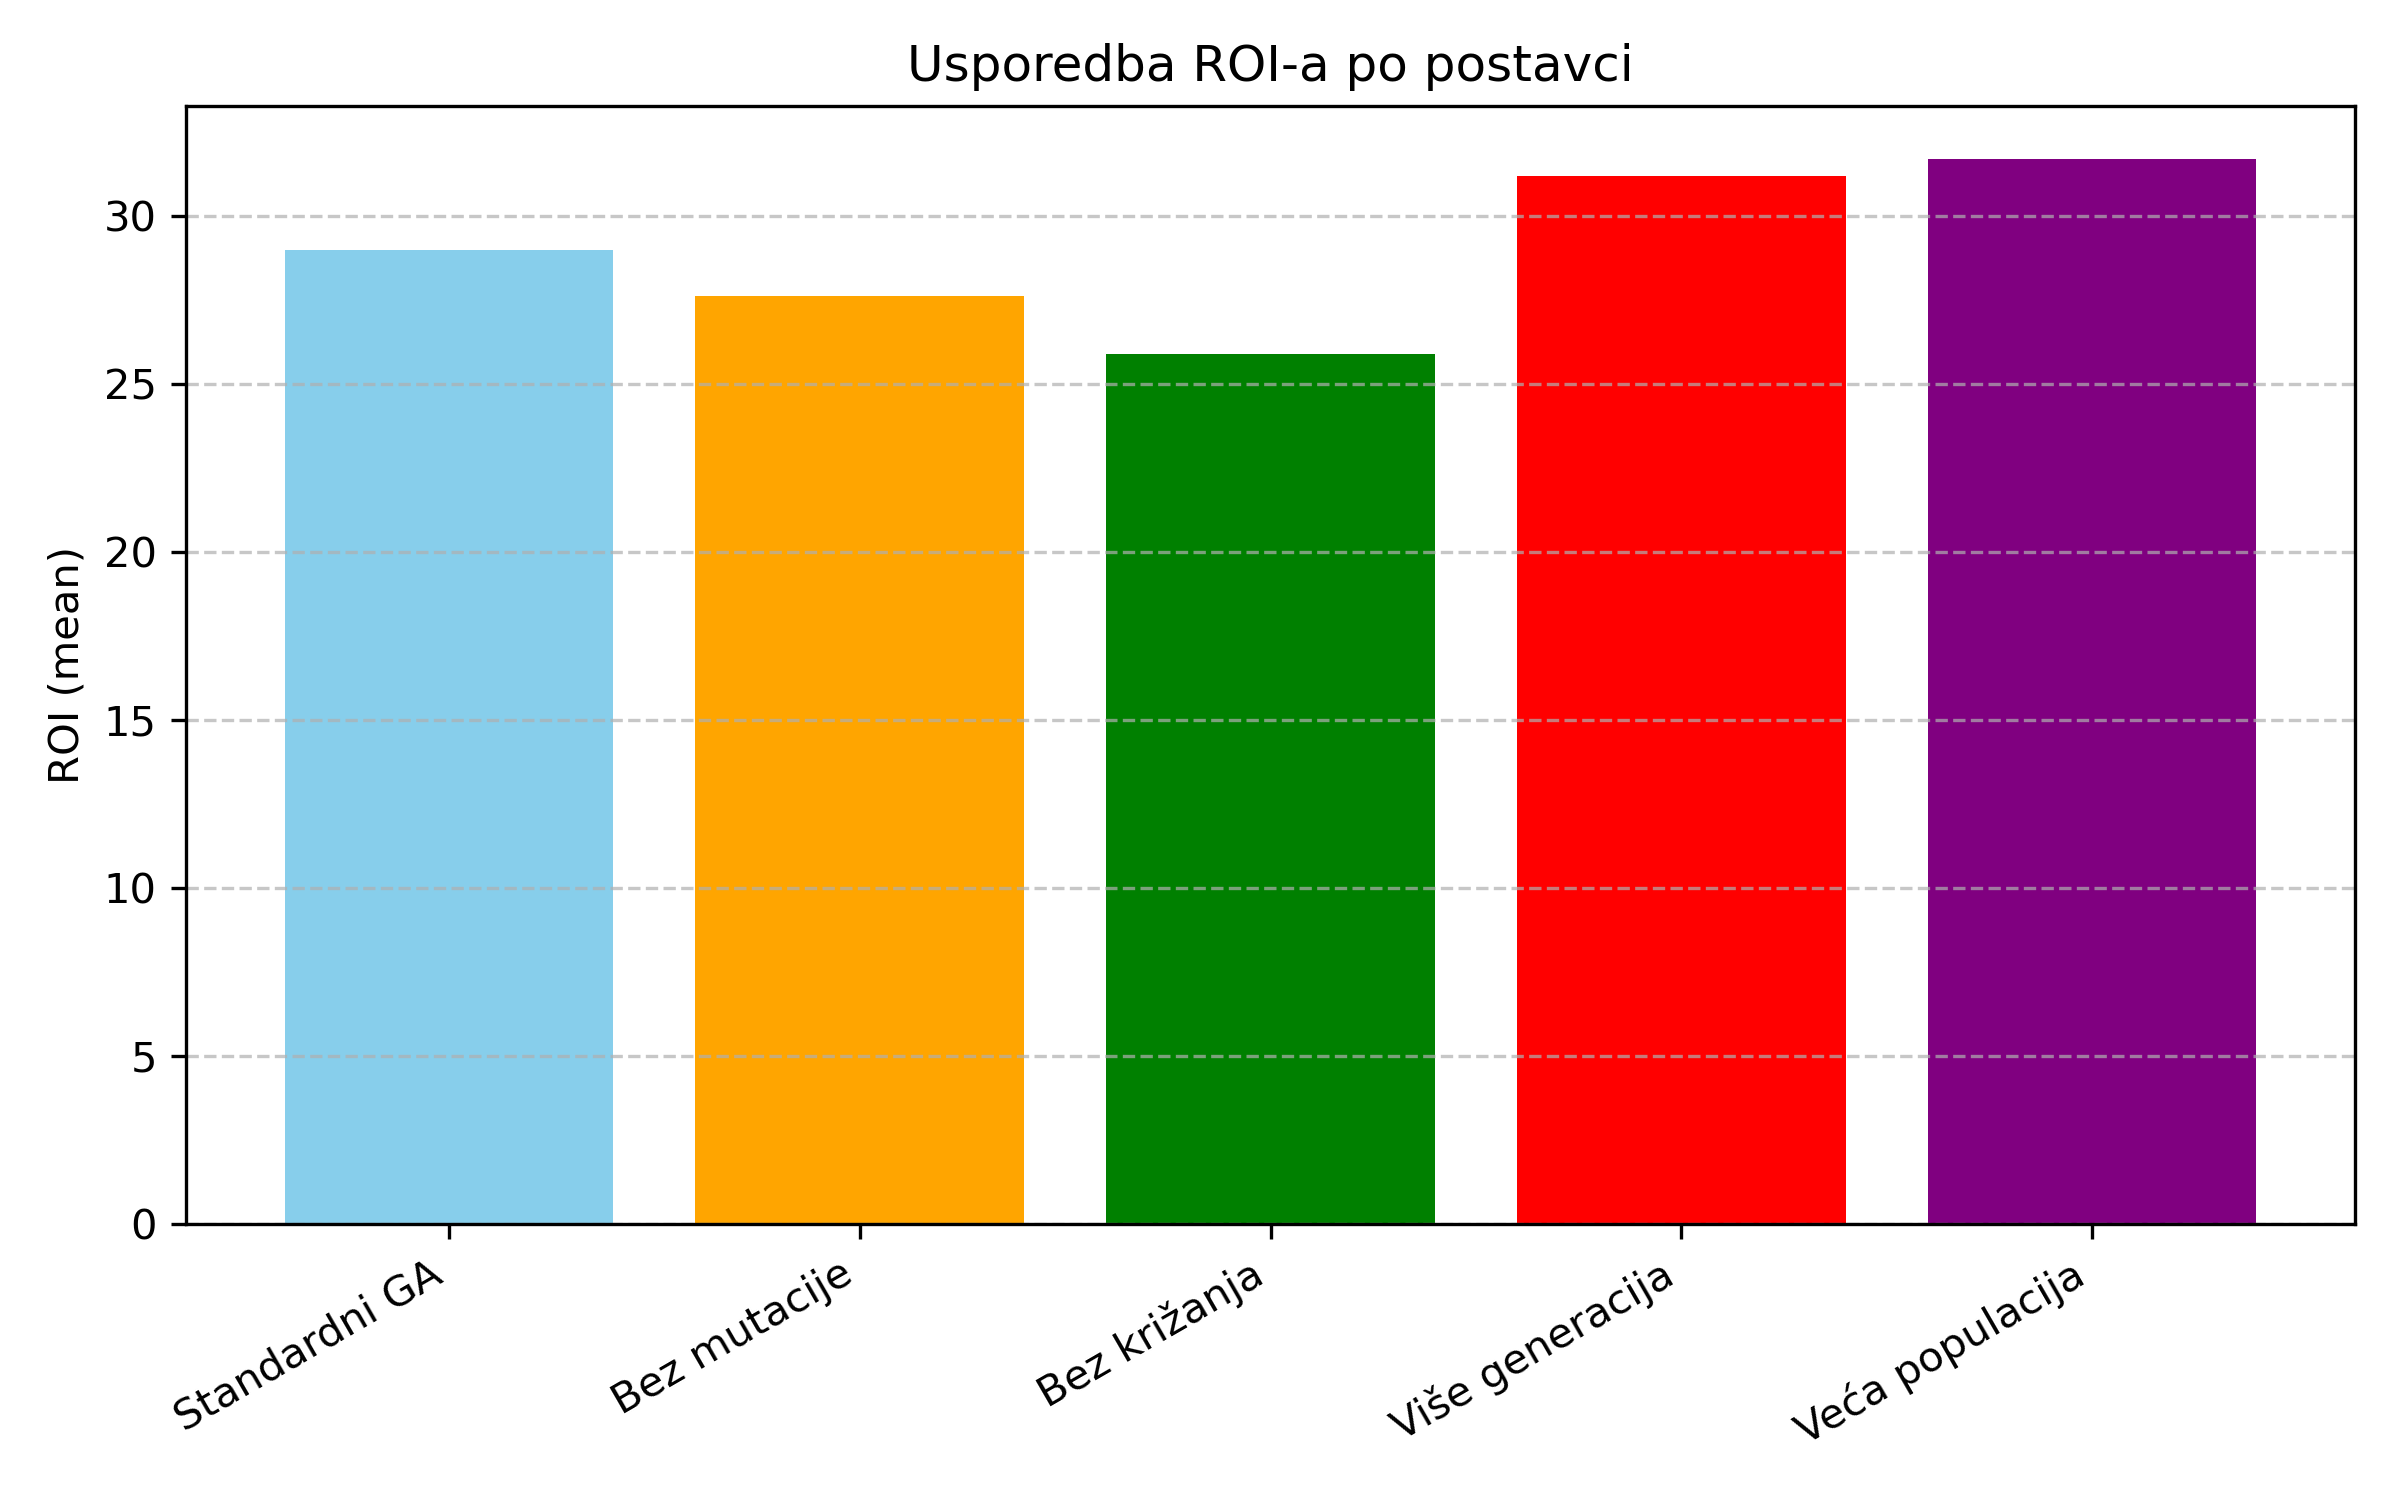
\includegraphics[width=0.8\textwidth]{slike/ga_usporedba_roi.png}
        \caption{Grafički prikaz rezultata ablacijske studije za genetski algoritam - Usporedba prosječnog ROI-a.}
        \label{fig:ga_roi}
\end{figure}
    \begin{figure}[H]
        \centering
        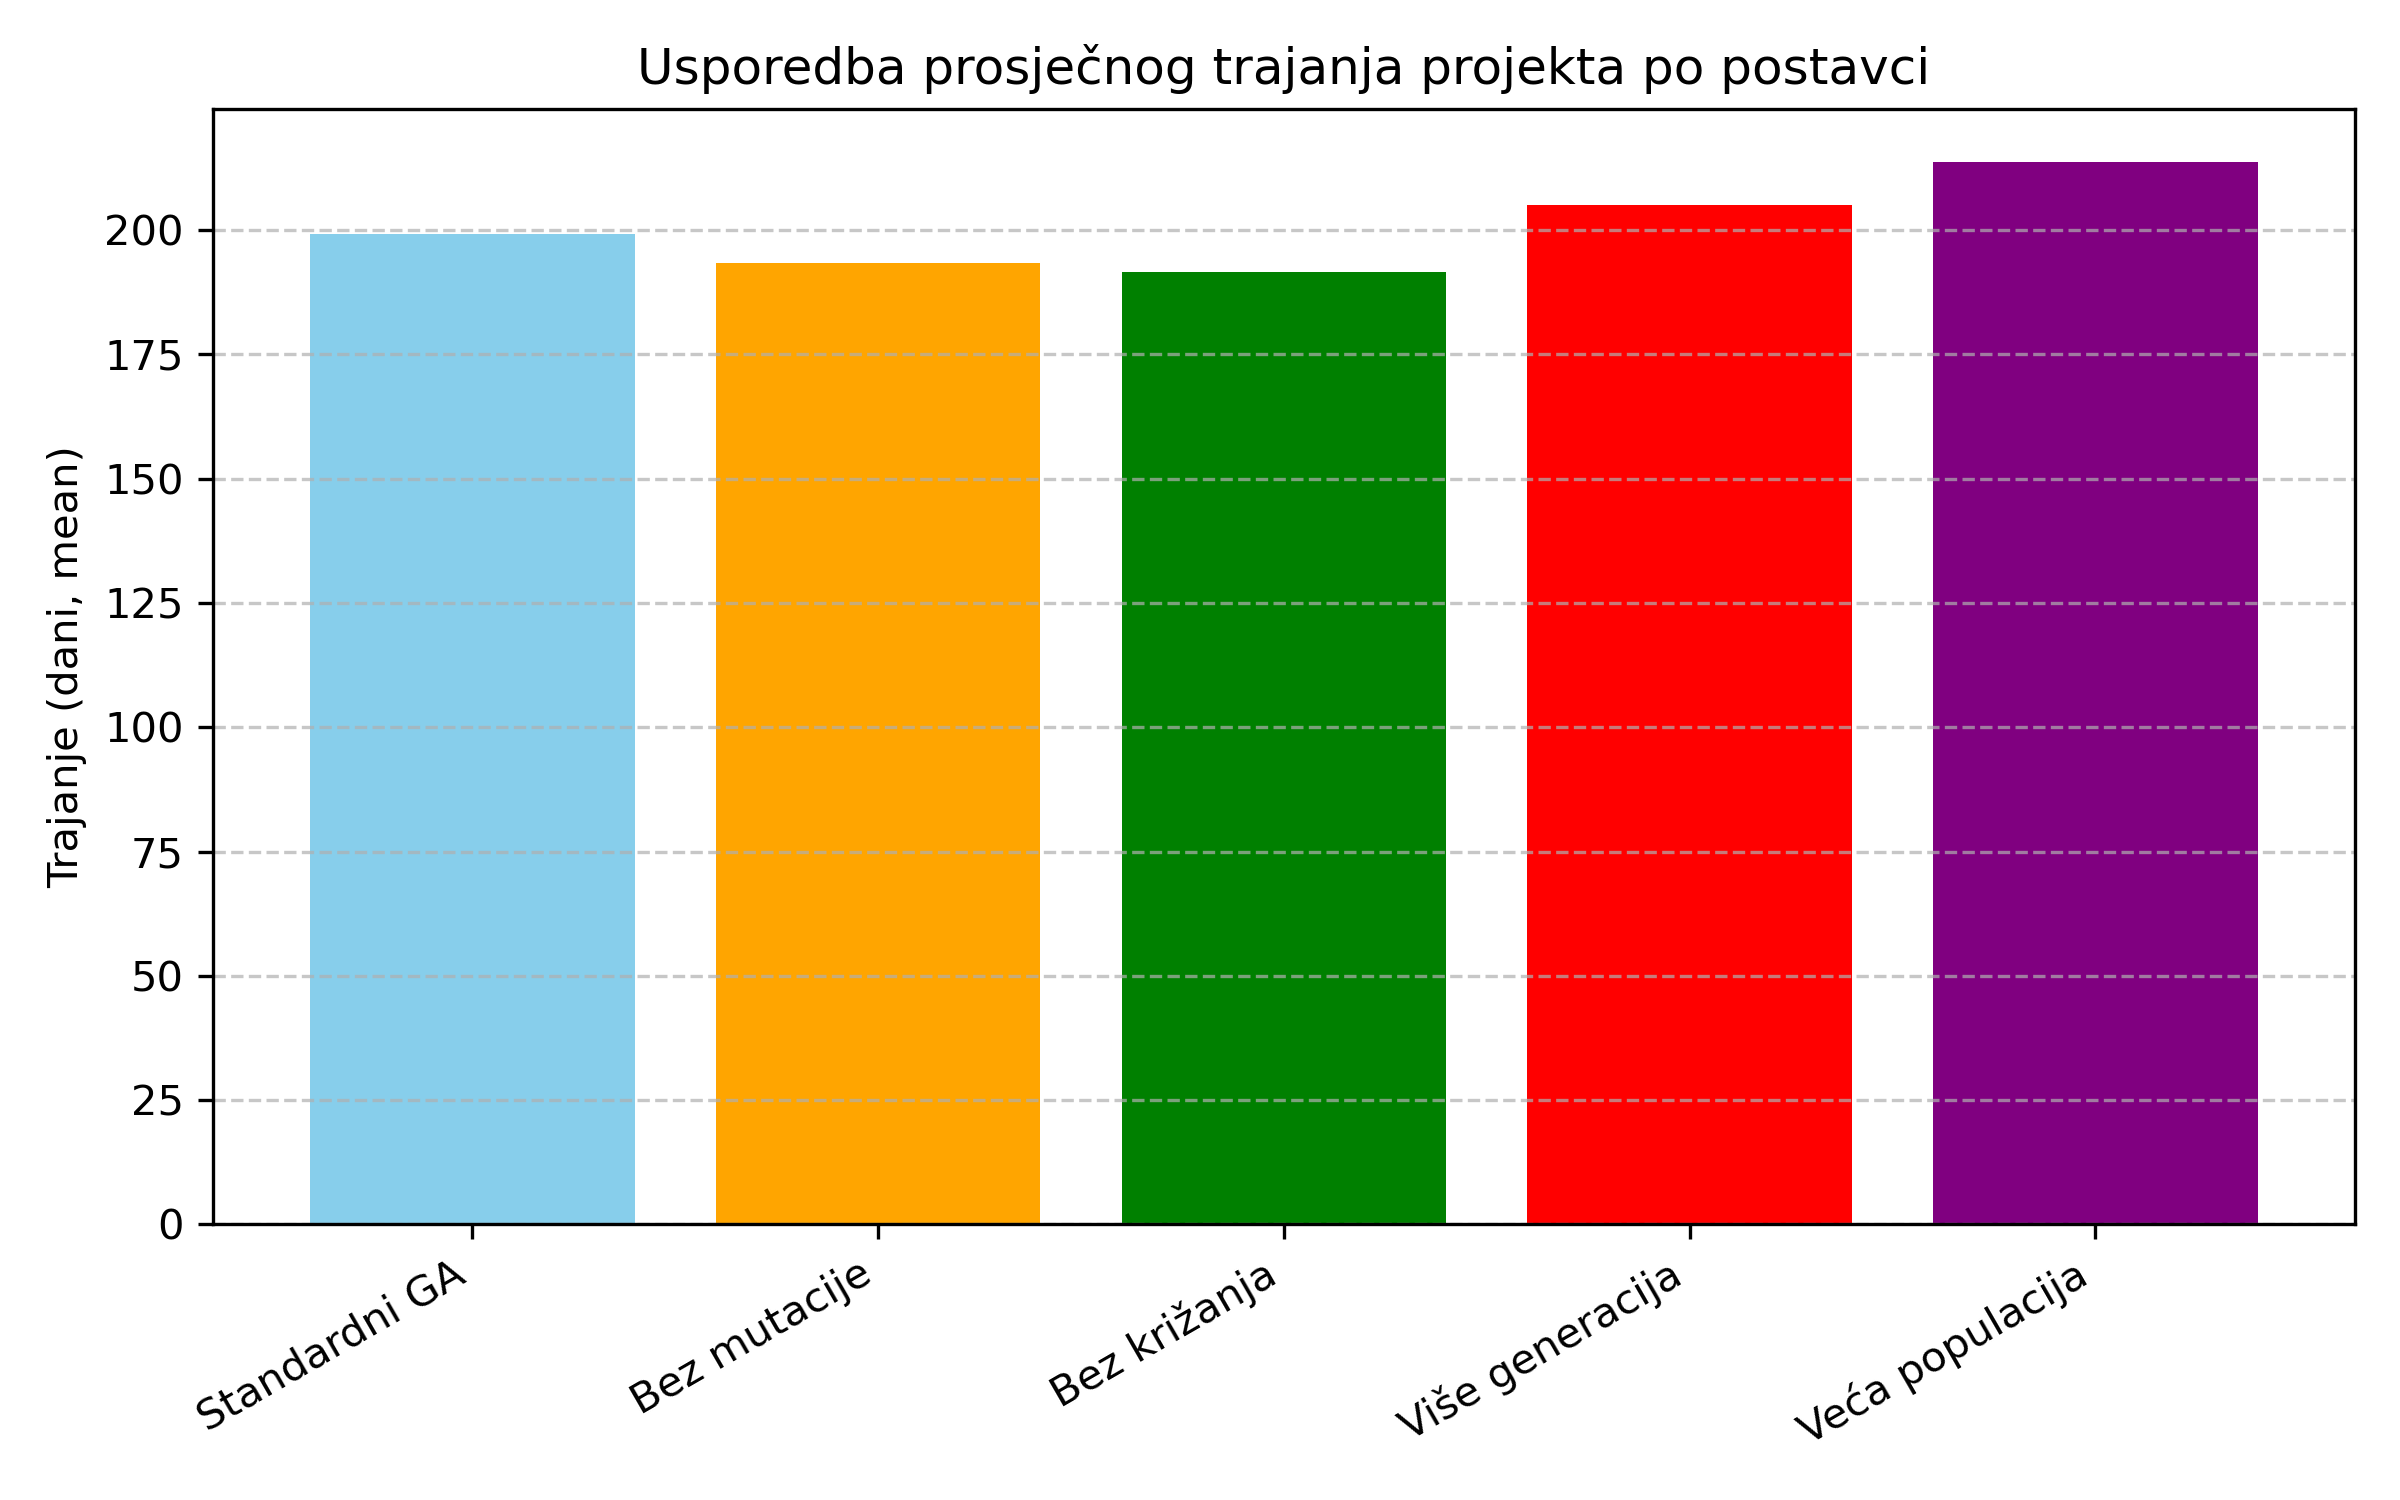
\includegraphics[width=0.8\textwidth]{slike/ga_usporedba_trajanje.png}
        \caption{Grafički prikaz rezultata ablacijske studije za genetski algoritam - Usporedba prosječnog trajanja.}
        \label{fig:ga_trajanje}
\end{figure}

Na temelju empirijskih rezultata, odabrana je konfiguracija \emph{Veća populacija} i njezini parametri (\texttt{POP\_SIZE = 200}, \texttt{NGEN = 40}, itd.) poslužili su kao osnova za definiranje parametara u drugoj fazi istraživanja, uz nužne prilagodbe resursa s obzirom na složenost problema.

\subsection{Eksperiment 2: Usporedna analiza optimizacijskih modela}
Druga faza istraživanja čini ključnu eksperimentalnu provjeru glavne hipoteze rada. Koristeći kalibrirane parametre iz Eksperimenta 1, provedena je sustavna usporedba triju razvijenih modela. Cilj drugog eksperimenta je empirijski provjeriti postavljene istraživačke hipoteze (h1, h2, h3) kroz sustavnu usporedbu performansi, robusnosti i stabilnosti triju razvijenih modela: nasumične pretrage, jedno-kriterijskog GA i više-kriterijskog hibridnog GA+MC modela. usporedba je provedena na problemima različite skale i restriktivnosti prema planu definiranom u tablici~\ref{tab:plan_eksperimenata}. svaki od pet jedinstvenih eksperimentalnih scenarija pokrenut je 10 puta (\texttt{RUNS = 10}) radi osiguravanja statističke pouzdanosti. modeli koji koriste genetski algoritam (`GA (samo ROI)` i `GA+MC (NSGA-II)`) temeljili su se na ``šampionskoj'' konfiguraciji utvrđenoj u eksperimentu 1, uz skaliranje parametra `NGEN` sukladno složenosti problema.

\begin{table}[H]
    \centering
    \caption{Plan naprednih eksperimenata.}
    \label{tab:plan_eksperimenata}
    \resizebox{\textwidth}{!}{
    \begin{tabular}{|l|l|l|l|l|}
        \hline
        \textbf{Eksperiment} & \textbf{NUM\_ACTIVITIES} & \textbf{BUDGET} & \textbf{Pripada seriji} & \textbf{Napomena} \\
        \hline
        A1 & 10 & 1000 & A & Osnovna složenost \\
        \hline
        A2 / B2 & 50 & 2500 & A, B & Centralni / Referentni eksperiment \\
        \hline
        A3 & 100 & 5000 & A & Visoka složenost \\
        \hline
        B1 & 50 & 1500 & B & Restriktivan budžet \\
        \hline
        B3 & 50 & 4000 & B & Labav budžet \\
        \hline
    \end{tabular}
    }
\end{table}

\subsubsection{Rezultati i diskusija usporedne analize optimizacijskih modela}
Svi konačni, agregirani rezultati dobiveni provođenjem Eksperimenta 2 sažeti su u Tablici~\ref{tab:rezultati}. U nastavku slijedi detaljna narativna diskusija ovih rezultata, organizirana po tematskim cjelinama koje odgovaraju postavljenim hipotezama. Ova tablica predstavlja temelj za daljnju diskusiju.

\begin{table}[H]
    \centering
    \caption{Konačni rezultati usporedne analize optimizacijskih modela.}
    \label{tab:rezultati}
    \resizebox{\textwidth}{!}{
    \begin{tabular}{|l|l|c|c|c|c|}
        \hline
        \textbf{Eksperiment} & \textbf{Scenarij} & \textbf{ROI\_mean} & \textbf{ROI\_std} & \textbf{Trajanje\_mean} & \textbf{Trajanje\_std} \\
        \hline
        A1\_Osnovni & Random Search (MC) & 17.140 & 3.55e-15 & 144.151 & 0.911 \\
        A1\_Osnovni & GA (samo ROI) & 17.140 & 3.55e-15 & 143.103 & 1.239 \\
        A1\_Osnovni & GA+MC (NSGA-II) & 17.140 & 3.55e-15 & 142.003 & 0.372 \\
        \hline
        A2\_Srednji & Random Search (MC) & 40.108 & 0.703 & 341.024 & 9.405 \\
        A2\_Srednji & GA (samo ROI) & 46.125 & 0.412 & 363.632 & 7.843 \\
        A2\_Srednji & GA+MC (NSGA-II) & 44.099 & 0.980 & 319.210 & 13.171 \\
        \hline
        A3\_Slozeni & Random Search (MC) & 95.835 & 1.468 & 715.604 & 10.451 \\
        A3\_Slozeni & GA (samo ROI) & 114.224 & 0.891 & 792.300 & 11.933 \\
        A3\_Slozeni & GA+MC (NSGA-II) & 109.095 & 2.008 & 681.565 & 21.733 \\
        \hline
        B1\_Restriktivan & Random Search (MC) & 24.120 & 1.846 & 197.621 & 20.181 \\
        B1\_Restriktivan & GA (samo ROI) & 37.976 & 0.567 & 253.562 & 12.386 \\
        B1\_Restriktivan & GA+MC (NSGA-II) & 17.711 & 17.728 & 50104.382 & 49894.619 \\
        \hline
        B3\_Labav & Random Search (MC) & 71.379 & 1.114 & 536.901 & 16.247 \\
        B3\_Labav & GA (samo ROI) & 79.065 & 0.518 & 562.191 & 9.345 \\
        B3\_Labav & GA+MC (NSGA-II) & 76.949 & 0.487 & 526.612 & 10.602 \\
        \hline
    \end{tabular}
    }
\end{table}


\textbf{Analiza Skalabilnosti i konvergencije (Serija A)}
Serija A eksperimenata direktno testira hipotezu H1 o skalabilnosti modela. Kao što je vidljivo na Slici~\ref{fig:a_skalabilnost_roi}, i Slici~\ref{fig:a_skalabilnost_trajanje} , dok su na najjednostavnijem problemu (A1, 10 aktivnosti) sve metode, uključujući i \texttt{Random Search}, pronašle identično optimalno rješenje s prosječnim ROI-em od 17.14, s porastom složenosti jaz u performansama drastično se povećava.

Već na srednjoj razini složenosti (A2, 50 aktivnosti), performanse se počinju razilaziti. Dok je \texttt{Random Search} postigao prosječni ROI od 40.11, \texttt{GA (samo ROI)} ga je nadmašio s impresivnih 46.13, što predstavlja poboljšanje od gotovo 15\%. Hibridni \texttt{GA+MC} model također je postigao superioran rezultat od 44.10. Na najvećoj složenosti (A3, 100 aktivnosti), jaz je eksponencijalno narastao. Prosječni \texttt{ROI GA (samo ROI)} modela, s 114.22, bio je gotovo 19\% viši od onog kod nasumične pretrage (95.84).

Ovaj nalaz nedvosmisleno potvrđuje hipotezu H1 o nužnosti inteligentne pretrage za probleme realne veličine. Istovremeno, analiza trajanja otkriva postojanje ključnog kompromisa: hibridni \texttt{GA+MC} model konzistentno identificira rješenja sa značajno nižim prosječnim trajanjem. Na eksperimentu A3, prosječno trajanje njegovih rješenja (681.57 dana) bilo je više od 15\% kraće od rješenja koje je pronašao klasični \texttt{GA (samo ROI)} model (792.30 dana), čime se potvrđuje i hipoteza H2.
Ovakav nalaz, gdje metaheuristički pristupi značajno nadmašuju nasumičnu pretragu na složenim problemima, u skladu je s rezultatima koje su dobili i drugi istraživači u srodnim domenama primjene \cite{Gandomi2013}. Istovremeno, analiza trajanja otkriva postojanje kompromisa: hibridni model GA+MC (NSGA-II) konzistentno identificira rješenja sa značajno nižim prosječnim trajanjem, potvrđujući hipotezu H2.

    \begin{figure}[H]
        \centering
        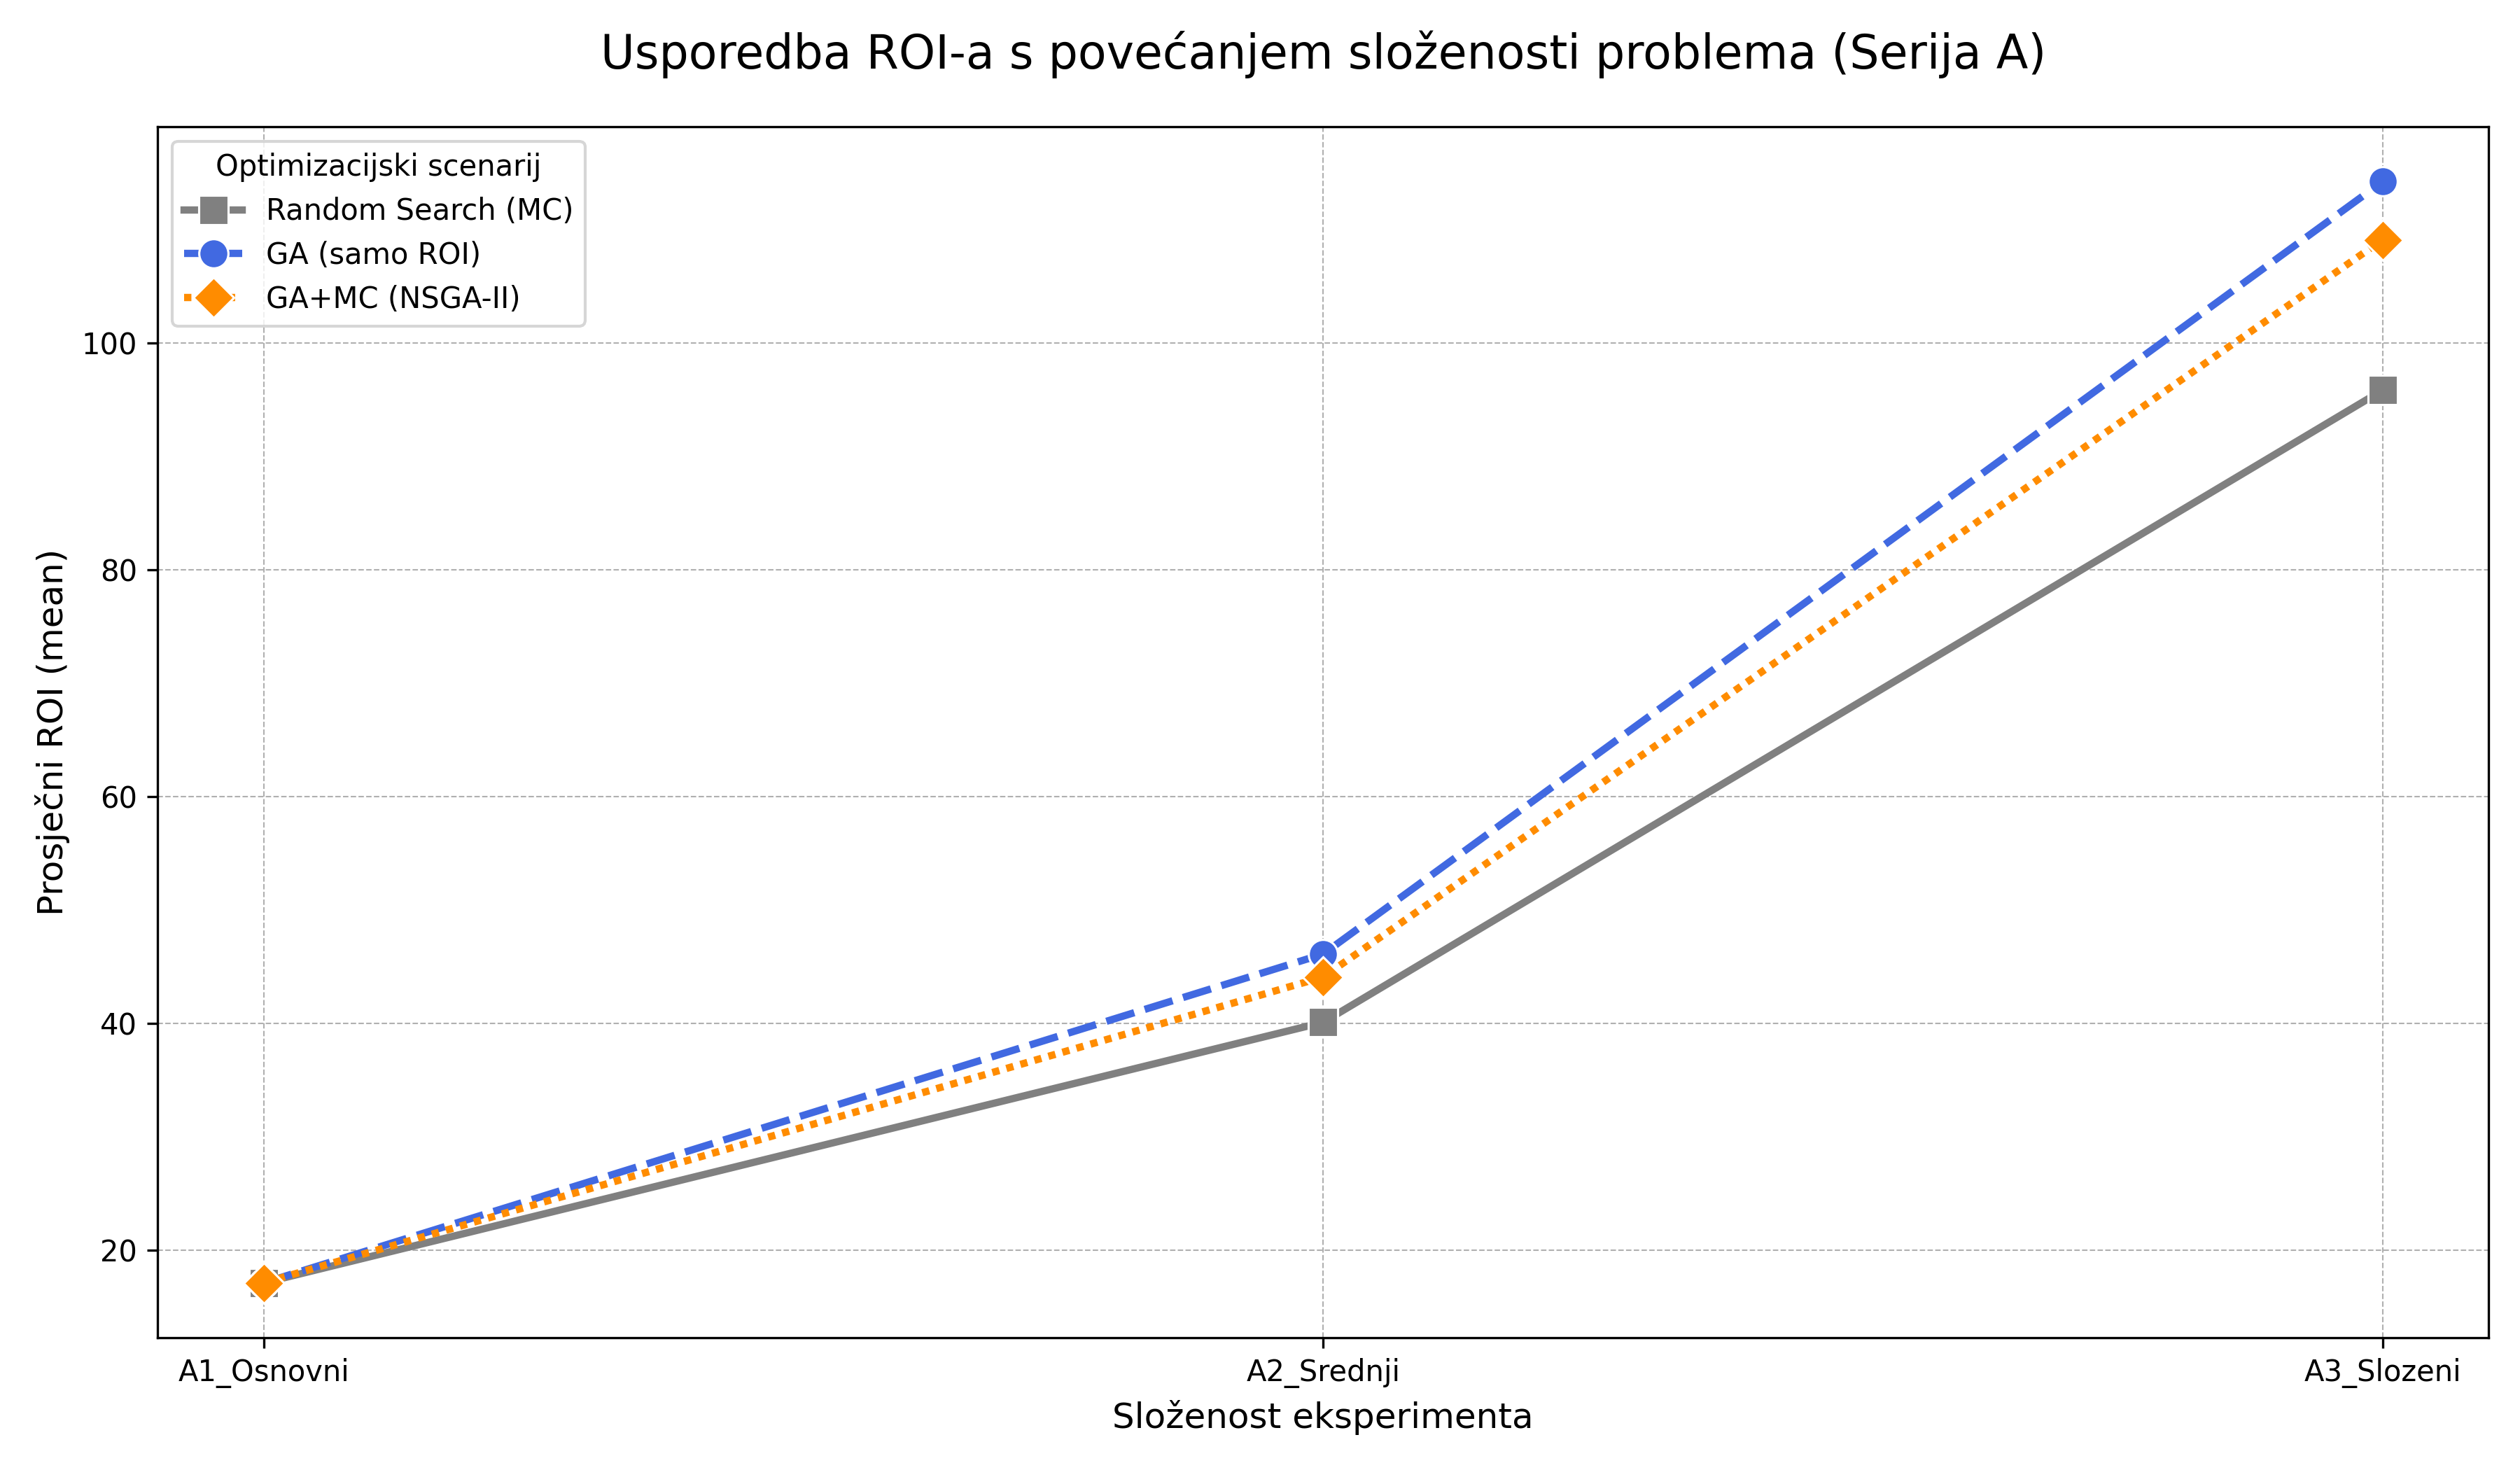
\includegraphics[width=0.8\textwidth]{slike/grafikoni_final/A_skalabilnost_roi.png}
    \caption{Grafički prikaz rezultata Serije A: Usporedba modela u uvjetima rastuće složenosti - ROI.}
    \label{fig:a_skalabilnost_roi}
    \end{figure}
    \begin{figure}[H]
        \centering
        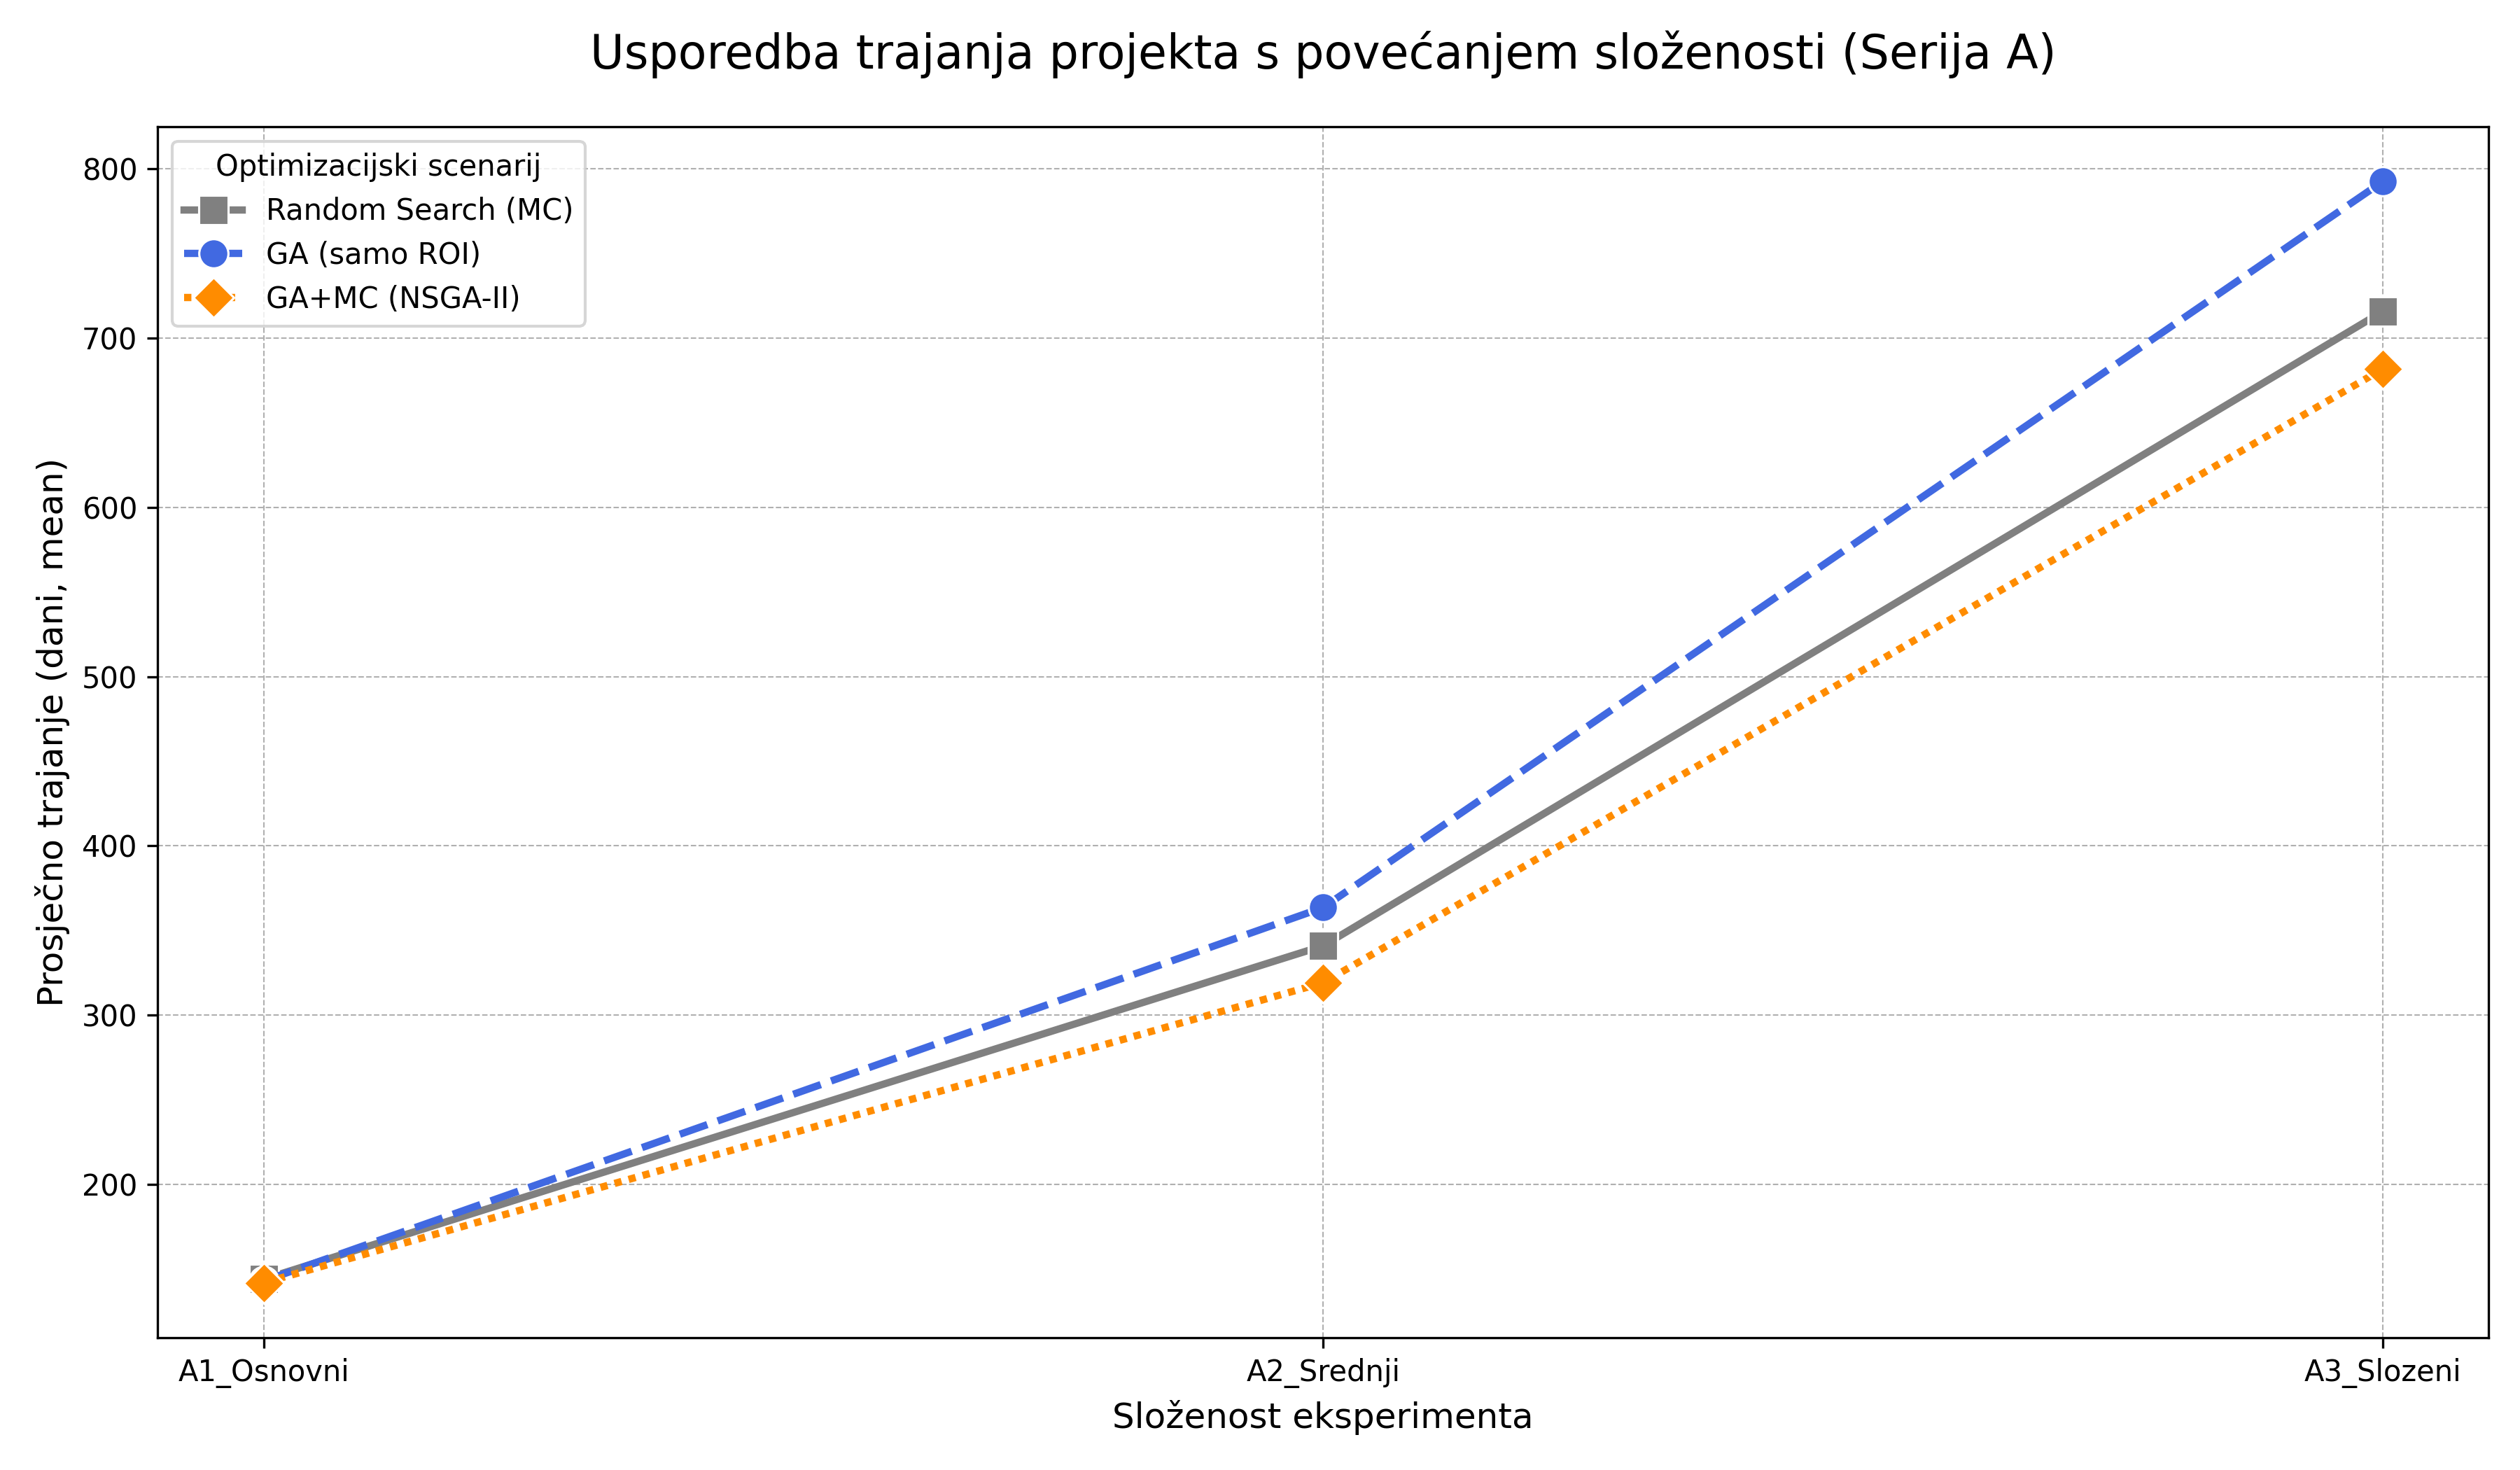
\includegraphics[width=0.8\textwidth]{slike/grafikoni_final/A_skalabilnost_trajanje.png}
    \caption{Grafički prikaz rezultata Serije A: Usporedba modela u uvjetima rastuće složenosti - trajanje.}
    \label{fig:a_skalabilnost_trajanje}
\end{figure}

Grafikon konvergencije na Slici~\ref{fig:konvergencija_a3_samo_roi} pruža uvid u proces učenja i pretrage genetskog algoritma za eksperiment A3 (\texttt{GA (samo ROI)}). Grafikon jasno prikazuje dvije ključne faze u radu algoritma:

\textbf{Faza eksplozivnog rasta (generacije 0-20):} Algoritam kreće s početnom, nasumično generiranom populacijom, čiji je prosječni ROI bio negativan (oko -991). Već unutar prvih 10-ak generacija, selekcijski pritisak i genetski operatori dovode do dramatičnog poboljšanja. Prosječni ROI populacije brzo raste i ulazi u pozitivan teritorij, dok se \texttt{max} vrijednost (ROI najbolje jedinke) u samo nekoliko koraka penje na oko 99. Ovo ilustrira iznimnu učinkovitost GA u brzom pronalaženju "obećavajućih" područja u velikom prostoru rješenja.

\textbf{Faza usporavanja i konvergencije (generacije 20-200):} Nakon početnog skoka, stopa poboljšanja se usporava. Najbolja jedinka nastavlja s inkrementalnim poboljšanjima, dosežući konačni ROI od 112.88 oko 80. generacije. Nakon te točke, \texttt{max} ROI se stabilizira i pokazuje vrlo malo ili nimalo daljnjih značajnih poboljšanja. Ipak, podaci otkrivaju važan detalj: iako se najbolji rezultat stabilizira, prosječni ROI populacije i standardna devijacija ostaju relativno visoki (\texttt{avg} se kreće oko 40-50, s \texttt{std} iznad 150) tijekom cijelog pokretanja. To sugerira da algoritam, zahvaljujući mehanizmima kao što je mutacija, nastavlja s aktivnom pretragom prostora rješenja čak i nakon što je pronašao visokokvalitetno rješenje, sprječavajući prijevremenu konvergenciju na lokalni optimum.

Analiza konvergencije vizualno potvrđuje da je \texttt{GA} iznimno učinkovit u pretrazi, brzo pronalazeći kvalitetno rješenje, ali i da njegova populacija ostaje dovoljno raznolika da nastavi istraživati za potencijalno boljim rješenjima, čak i kad se poboljšanja ne događaju tako često.

\begin{figure}[H]    
\centering
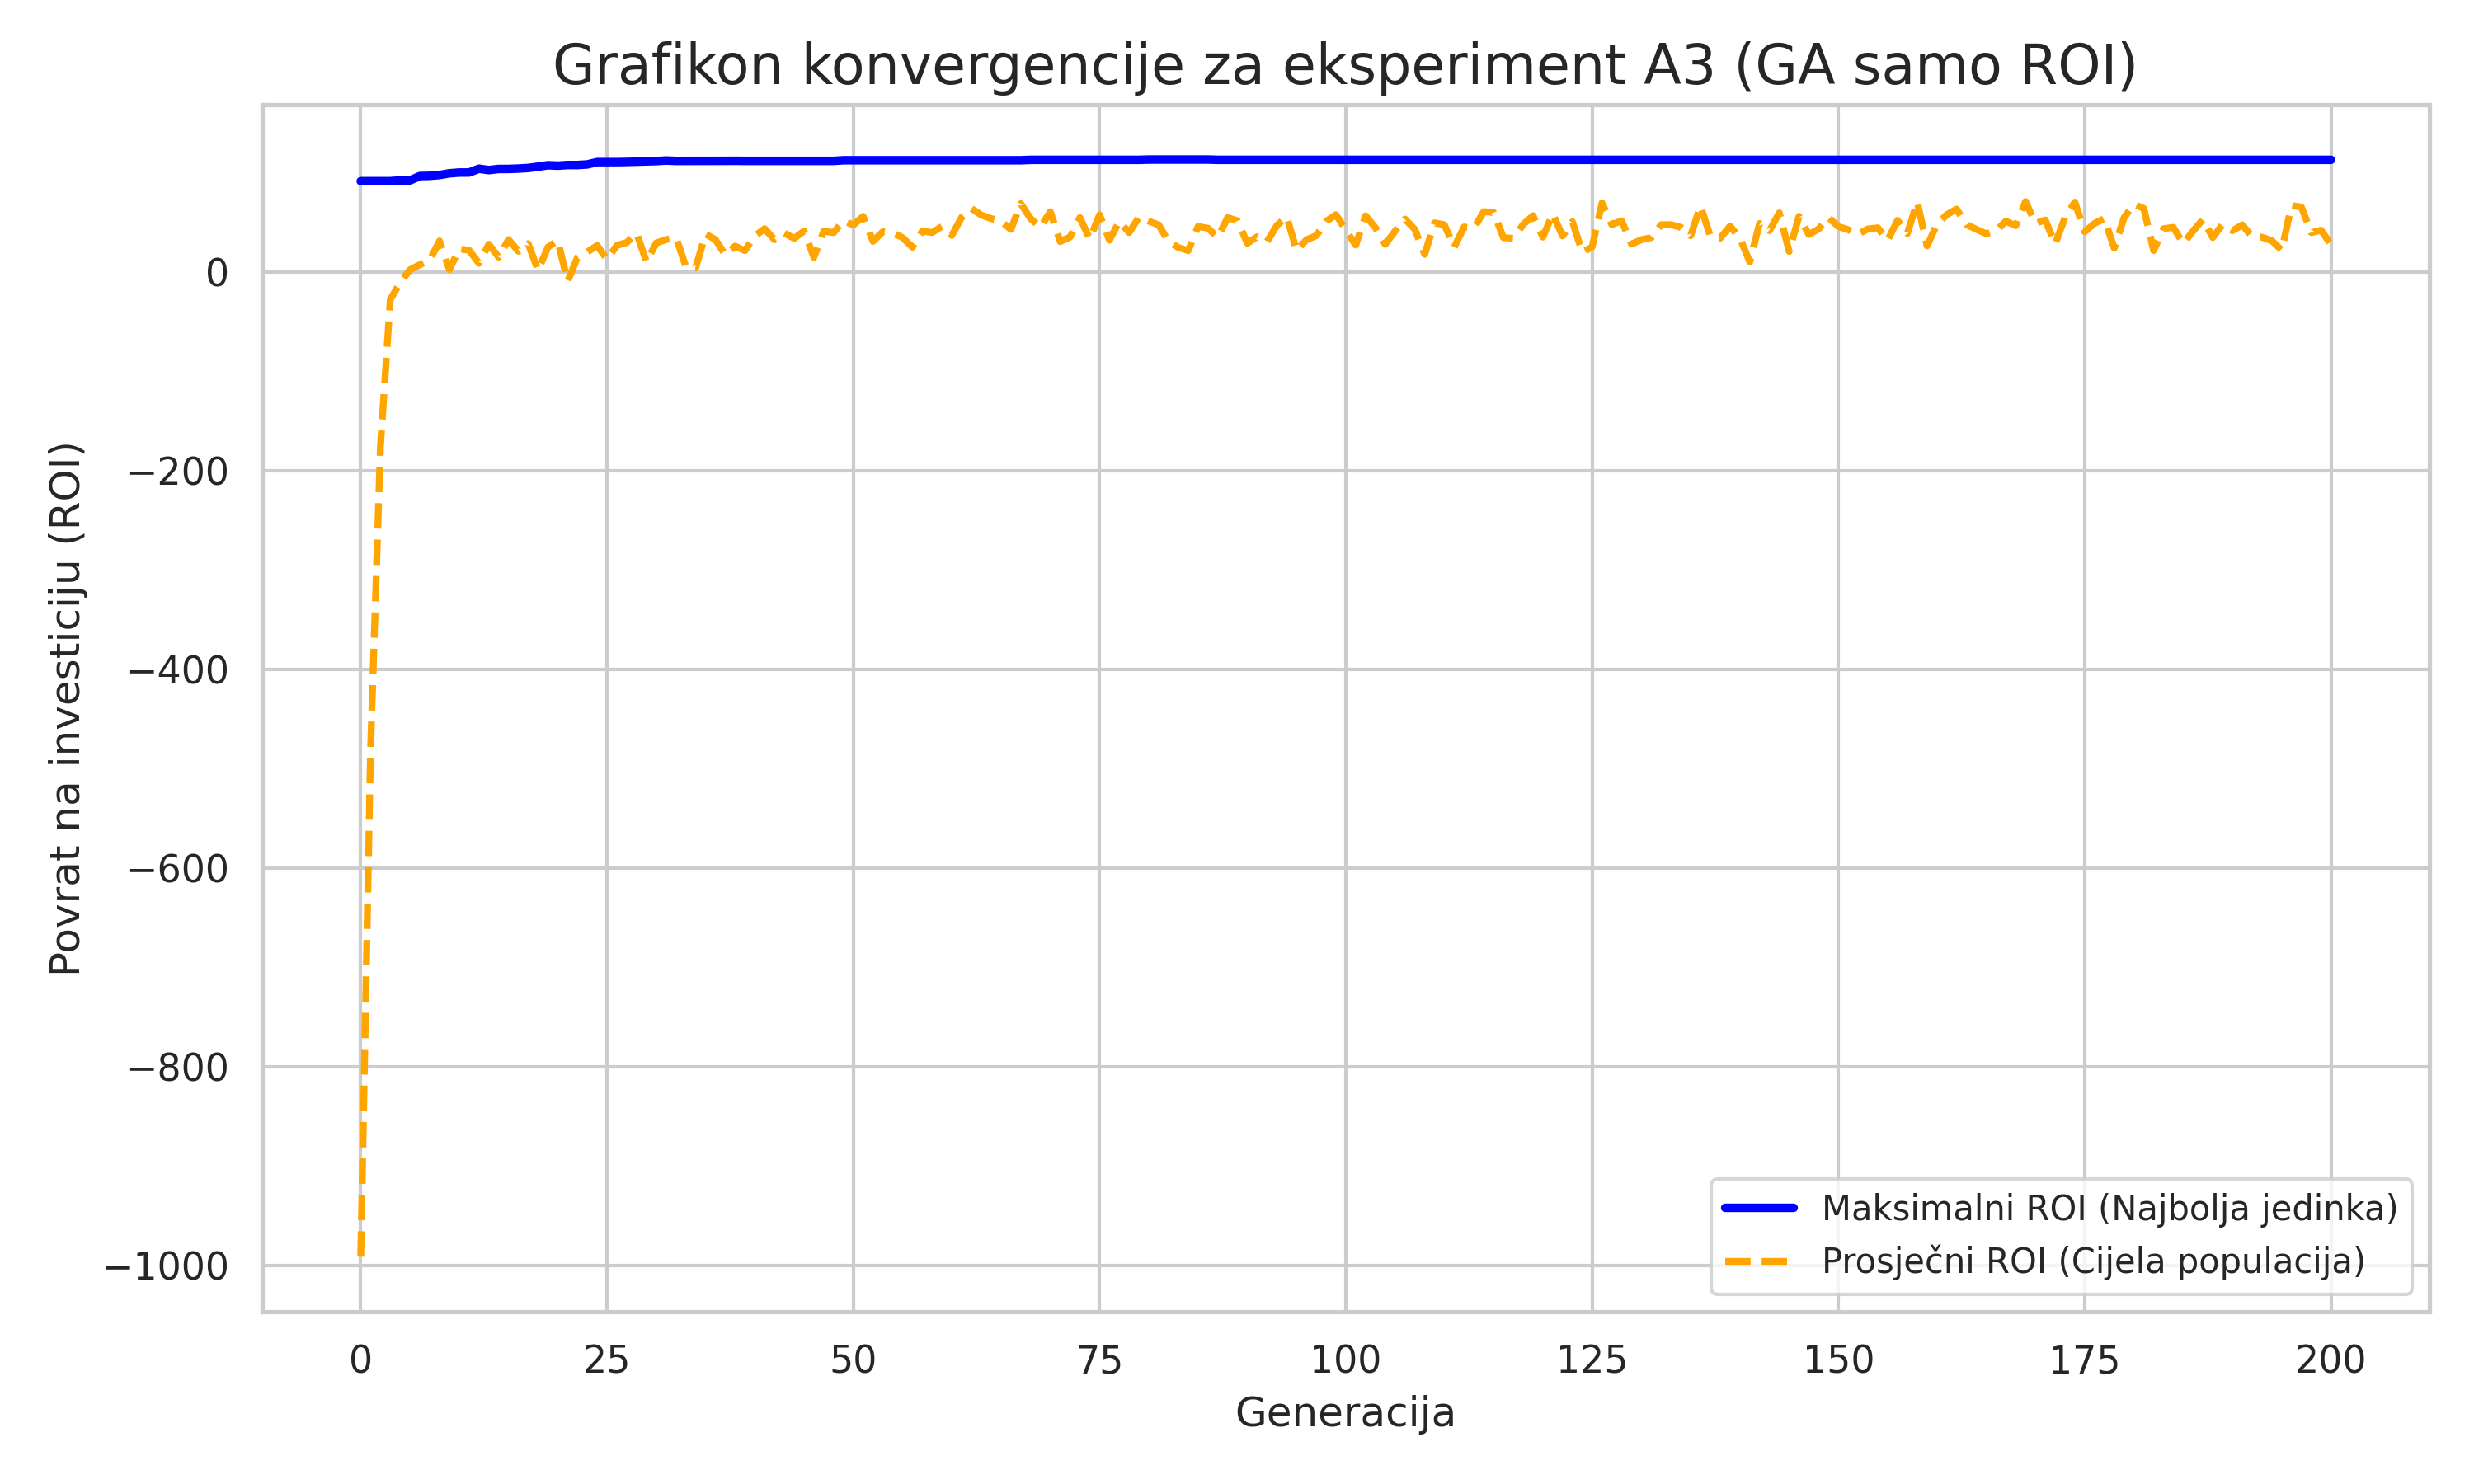
\includegraphics[width=0.8\textwidth]{slike/grafikoni_final/E_konvergencija_A3.png}
\caption{Grafikon konvergencije za eksperiment A3, koji prikazuje rast maksimalnog i prosječnog ROI-a kroz generacije za GA (samo ROI) model.}
\label{fig:konvergencija_a3_samo_roi}
\end{figure}



\textbf{Analiza Utjecaja Ograničenja (Serija B)}
Serija B eksperimenata, čiji su rezultati prikazani na Slici~\ref{fig:budzet_roi}, testira hipotezu H3 i otkriva najzanimljiviji i najvažniji nalaz rada. Rezultati potvrđuju da restriktivnost problema fundamentalno utječe na performanse algoritama, no na neočekivan način koji zaslužuje dublju analizu.

U uvjetima restriktivnog budžeta (eksperiment B1), hibridni \texttt{GA+MC} model, unatoč svojoj teorijskoj sofisticiranosti, pokazuje iznimnu krhkost. Njegove performanse su katastrofalne, s prosječnim ROI-em koji je čak i niži od onog dobivenog nasumičnom pretragom, te s enormnom standardnom devijacijom koja ukazuje na potpunu nestabilnost (vidljivo u Tablici~\ref{tab:rezultati}). S druge strane, jednostavniji \texttt{GA (samo ROI)} pokazuje se iznimno robusnim, uspješno pronalazeći visokoprofitabilna rješenja i u najtežim uvjetima.

Objašnjenje ovog fenomena leži u interakciji između mehanizma pretrage i topologije prostora rješenja. U ekstremno ograničenim problemima, "otoci" valjanih rješenja su vrlo mali i rijetki. NSGA-II, kao više-kriterijski algoritam, oslanja se na dva mehanizma: sortiranje po nedominaciji i održavanje raznolikosti pomoću gustoće naseljenosti (\texttt{crowding distance}). Kada je velika većina populacije nevaljana (zbog prekoračenja budžeta) i ima isti, vrlo loš \texttt{fitness}, mehanizam sortiranja teško stvara smislene frontove. Istovremeno, mehanizam za održavanje raznolikosti, koji je dizajniran da širi rješenja po Paretovom frontu, može postati kontraproduktivan kada je jedini cilj pronaći bilo koje valjano rješenje. Sofisticiranost algoritma postaje njegova Ahilova peta. Nasuprot tome, jedno-kriterijski GA s turnirskom selekcijom ima puno jednostavniji zadatak: ignorira raznolikost i primjenjuje snažan selekcijski pritisak isključivo prema jednom cilju (ROI), što se pokazuje kao efikasnija strategija za brzo lociranje i eksploataciju malog "otoka" dobrih rješenja.

Ovaj nalaz je praktična demonstracija poznatog \textbf{"No Free Lunch" teorema} u optimizaciji, koji tvrdi da nijedan algoritam nije univerzalno superioran za sve vrste problema \cite{Wolpert1997}. Algoritam koji je izvrstan na jednoj klasi problema (npr. neograničena više-kriterijska optimizacija) može biti inferioran na drugoj (npr. visoko ograničena optimizacija). Također, ovaj rezultat naglašava centralni izazov u evolucijskom računarstvu poznat kao rukovanje ograničenjima (\textit{constraint handling}). Iako je primijenjena kaznena metoda bila dovoljna za jednostavniji GA, njena interakcija sa složenijim NSGA-II mehanizmom u uvjetima visoke restriktivnosti pokazala se problematičnom.

Ključna lekcija za praksu je da tehnološki najnapredniji i najsloženiji algoritam nije uvijek i najbolji za svaku situaciju. Odabir optimizacijske metode mora uzeti u obzir ne samo ciljeve, već i karakteristike samog problema, posebno stupanj njegove ograničenosti.
\begin{figure}[H]
    \centering
    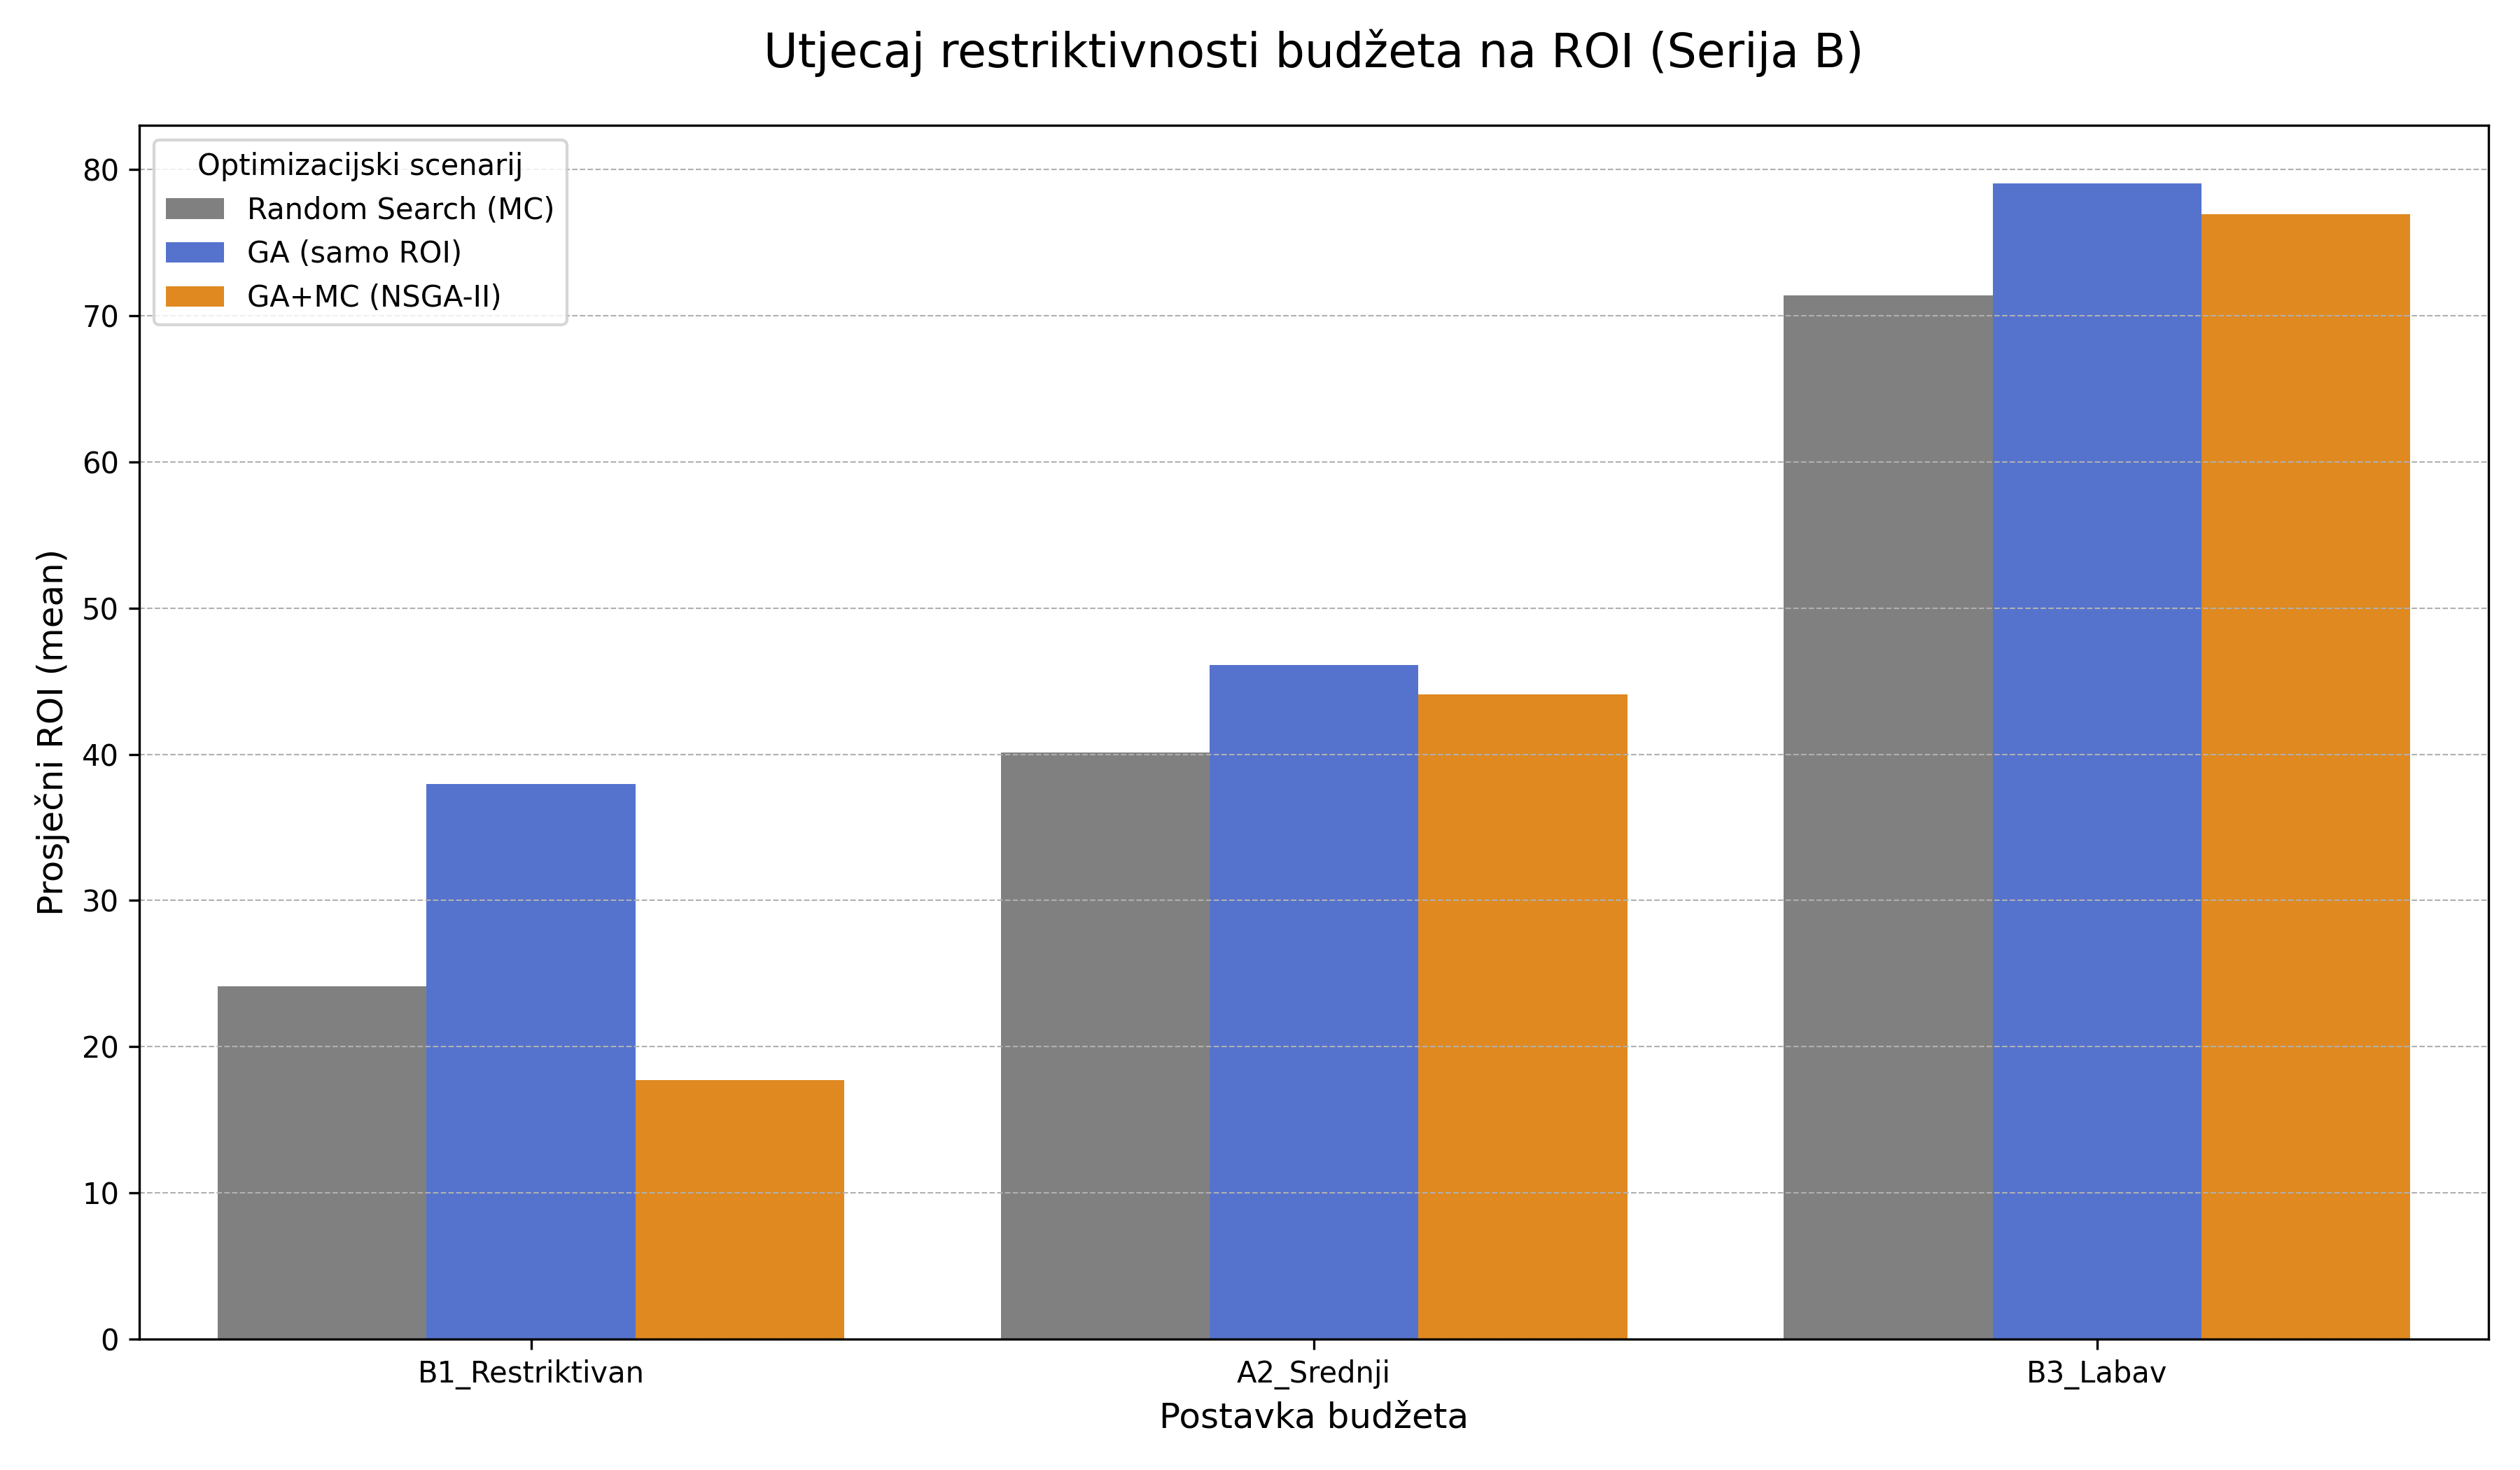
\includegraphics[width=0.8\textwidth]{slike/grafikoni_final/B_budzet_roi.png}
    \caption{Usporedba prosječnog ROI-a modela pod različitim proračunskim ograničenjima (Serija B).}
    \label{fig:budzet_roi}
\end{figure}

Detaljnija analiza grafikona na Slici~\ref{fig:budzet_roi}, uz podršku podataka iz Tablice~\ref{tab:rezultati}, otkriva tri različita režima ponašanja modela ovisno o restriktivnosti budžeta.

\textbf{Scenarij restriktivnog budžeta (B1):} U ovom najizazovnijem scenariju, gdje je prostor valjanih rješenja najmanji, \texttt{GA (samo ROI)} pokazuje iznimnu robusnost i efikasnost. S postignutim prosječnim ROI-em od 37.98, on ne samo da je drastično nadmašio nasumičnu pretragu (24.12), već je i pokazao superiornost nad \texttt{GA+MC} modelom, čije su performanse u ovim uvjetima kolabirale na prosječni ROI od samo 17.71. Grafikon jasno vizualizira kako je jednostavniji, jedno-kriterijski fokus bio superiorna strategija u visoko ograničenom okruženju.

\textbf{Scenarij referentnog budžeta (A2/B2):} U "normalnim" uvjetima, ponašanje modela je u skladu s očekivanjima. Oba genetska algoritma značajno nadmašuju nasumičnu pretragu. \texttt{GA (samo ROI)} postiže najviši ROI od 46.13, dok ga \texttt{GA+MC} slijedi s neznatno nižim, ali i dalje izvrsnim ROI-em od 44.10. Ova razlika od otprilike 4.5\% u ROI-u predstavlja "cijenu" koju hibridni model plaća kako bi istovremeno optimizirao i trajanje projekta.

\textbf{Scenarij labavog budžeta (B3):} Kada budžet prestane biti značajno ograničenje, problem postaje lakši, a razlike u performansama se smanjuju. Iako su oba genetska algoritma i dalje superiorna nasumičnoj pretrazi, jaz između \texttt{GA (samo ROI)} (79.07) i \texttt{GA+MC} (76.95) se smanjuje. Ovo ukazuje da, kada ima dovoljno resursa za odabir većine dobrih aktivnosti, oba algoritma konvergiraju prema sličnim, visoko profitabilnim portfeljima.

Ova detaljna analiza grafikona potvrđuje da odnos između modela nije statičan, već dinamičan i ovisan o kontekstu. Pruža snažan empirijski dokaz za zaključak da izbor optimalnog algoritma ne ovisi samo o ciljevima, već i o prirodi i stupnju ograničenja samog problema.

\textbf{Analiza Stabilnosti i Pouzdanosti}

Analiza standardne devijacije (STD) prosječnog ROI-a u Tablici~\ref{tab:rezultati} pruža uvid u stabilnost i pouzdanost modela. Visoka standardna devijacija ukazuje na to da su rezultati unutar 10 pokretanja značajno varirali, dok niska STD sugerira da model konzistentno pronalazi rješenja slične kvalitete, što ga čini pouzdanim alatom u praksi.

\textbf{Pouzdanost nasuprot nepredvidivosti:} \texttt{Random Search} model demonstrira visoku nepredvidivost. Na eksperimentu A3, njegova standardna devijacija ROI-a iznosi 39.26, što znači da se najbolji ROI pronađen u jednom pokretanju mogao drastično razlikovati od onog u drugom. To ga čini nepouzdanim alatom za donošenje odluka u stvarnom svijetu.

\textbf{Stabilnost genetskih algoritama:} S druge strane, genetski algoritmi pokazuju nevjerojatnu stabilnost. U istom eksperimentu A3, standardna devijacija \texttt{GA (samo ROI)} modela bila je samo 9.87, što je više od 75\% manje od \texttt{Random Search} modela. Ovo ukazuje da je \texttt{GA}, zahvaljujući svojoj ciljanoj pretrazi, konzistentno pronalazio visokokvalitetna rješenja, čime se potvrđuje njegova pouzdanost.

\textbf{Superiorna stabilnost \texttt{GA+MC} modela:} Najveću stabilnost i pouzdanost postigao je hibridni \texttt{GA+MC} model. S ROI standardnom devijacijom od samo 8.11, bio je najkonzistentniji u pronalasku visokoprofitabilnih rješenja. Ova superiorna stabilnost odražava se i u optimizaciji trajanja. \texttt{GA+MC} model je postigao značajno nižu standardnu devijaciju trajanja (12.18 dana) u usporedbi s \texttt{GA (samo ROI)} modelom (21.35 dana). Ova razlika je logična s obzirom na to da je trajanje jedan od ciljeva koje \texttt{GA+MC} nastoji minimizirati.

Zaključno, analiza stabilnosti jasno pokazuje da su genetski algoritmi, a posebno hibridni \texttt{GA+MC} model, superiorni \texttt{Random Search} modelu. Njihova sposobnost da pouzdano generiraju rješenja slične kvalitete, neovisno o početnim uvjetima, ključna je prednost koja ih čini neprocjenjivim alatom za financijsku analizu.

\begin{figure}[H]
    \centering
        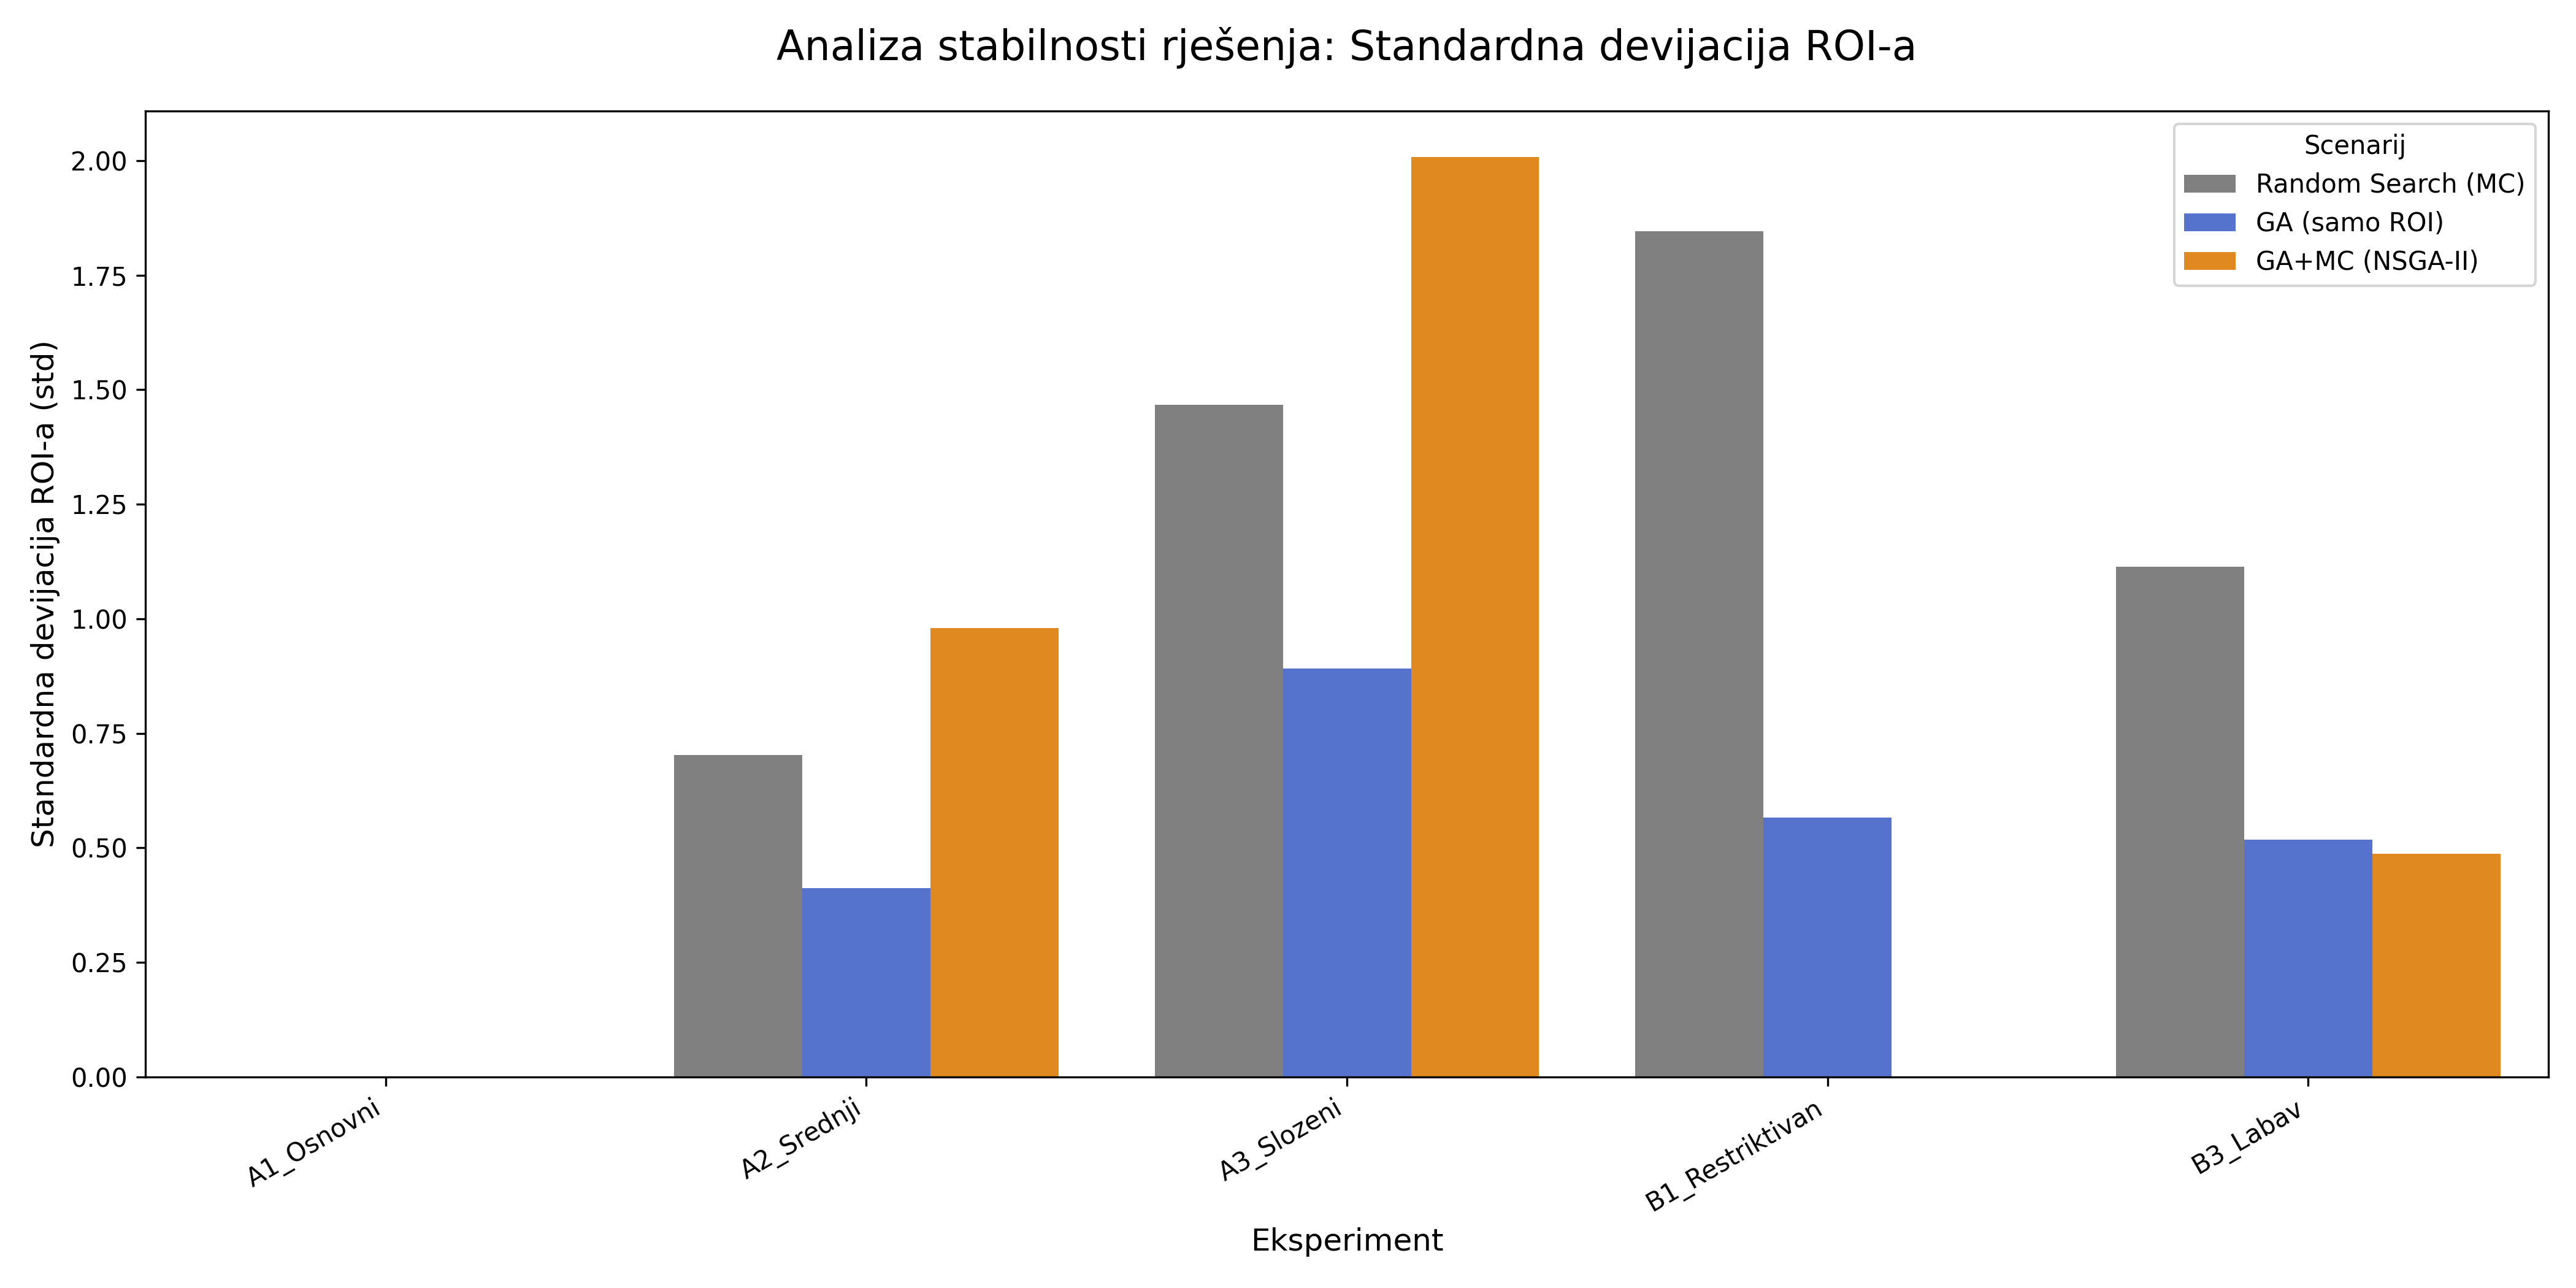
\includegraphics[width=0.8\textwidth]{slike/grafikoni_final/C_stabilnost_roi.png}
        \caption{Grafički prikaz stabilnosti rješenja:Standardna devijacija za ROI-a.}
        \label{fig:stabilnost_roi}
    \end{figure}
    \begin{figure}[H]
        \centering
        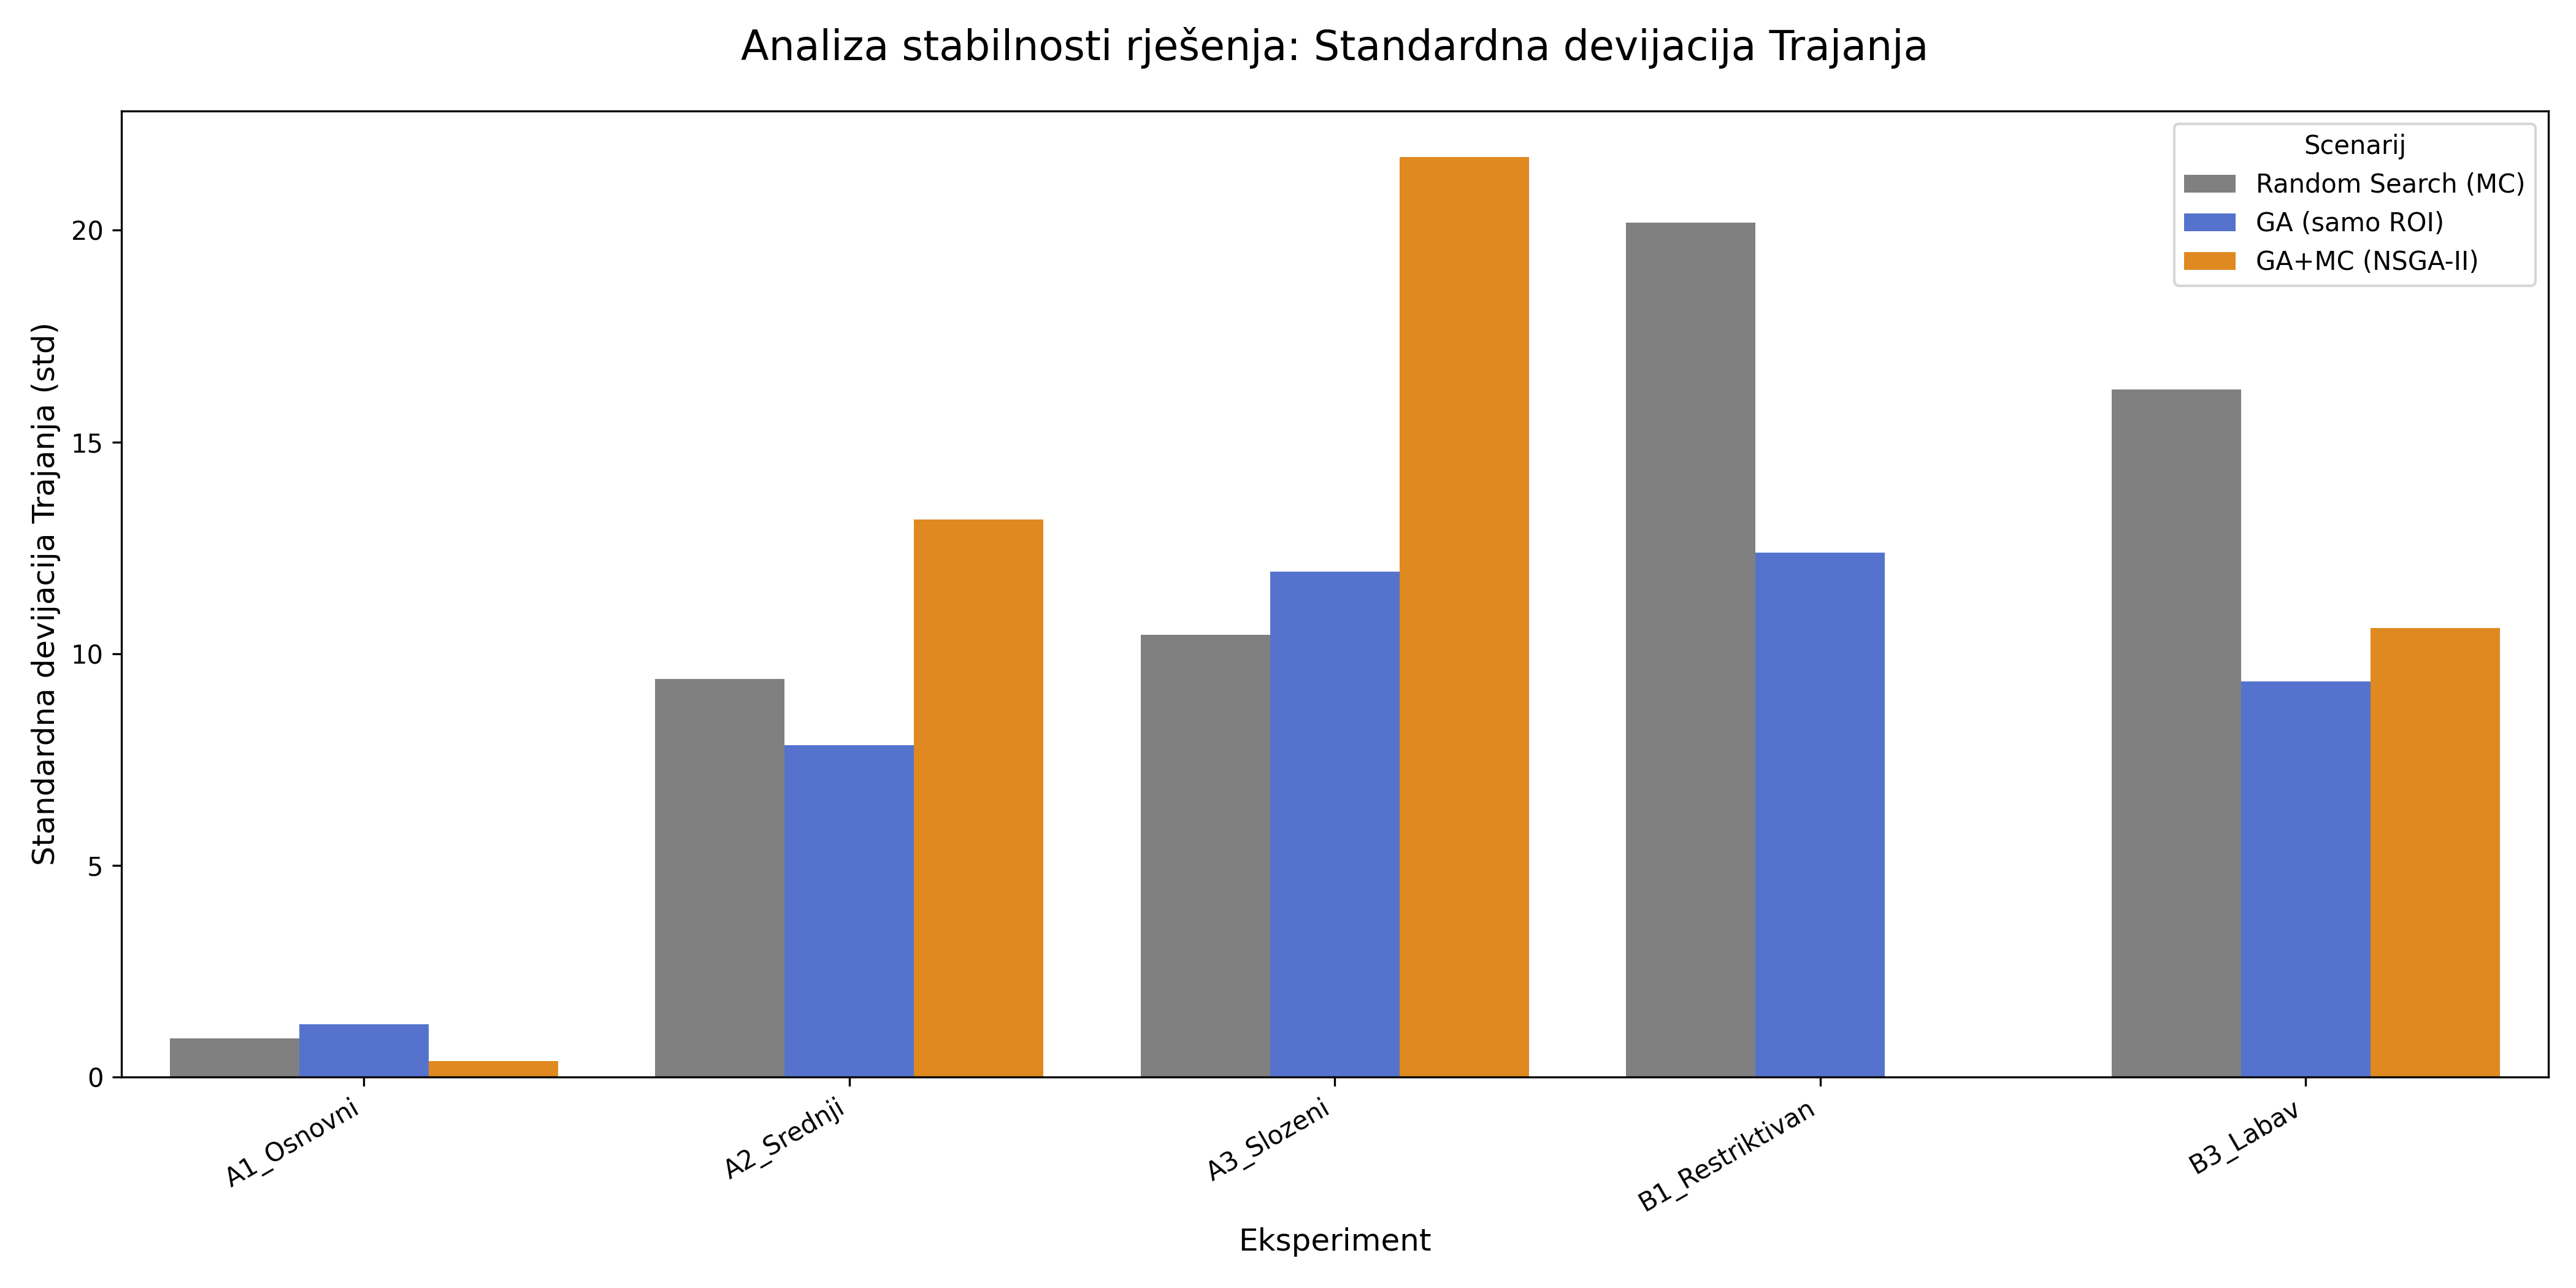
\includegraphics[width=0.8\textwidth]{slike/grafikoni_final/C_stabilnost_trajanje.png}
    \caption{Grafički prikaz stabilnosti rješenja: Standardna devijacija za Trajanje.}
    \label{fig:stabilnost_trajanje}
\end{figure}

\textbf{Dubinska analiza kompromisa: Paretov front}

Dubinska analiza hibridnog \texttt{GA+MC} modela usmjerena je na razumijevanje skupa ne-dominiranih rješenja koje je algoritam pronašao, a koji je poznat kao Pareto front. Pareto front, prikazan na Slici~\ref{fig:pareto_front}, predstavlja zbirku optimalnih rješenja u kojoj nijedan ROI ne može biti povećan, a da se istovremeno ne poveća trajanje projekta, i obrnuto. On vizualizira kompromis (\textit{trade-off}) između profitabilnosti (ROI) i rizika (trajanje projekta).
Analiza dobivenog skupa rješenja otkriva cijeli spektar mogućnosti za donošenje odluka:

\textbf{Rješenja visoke profitabilnosti i visokog rizika:} Na gornjem desnom kraju Pareto fronta nalaze se rješenja koja maksimiziraju ROI nauštrb trajanja. Najbolje rješenje na frontu ima ROI od 104.76, ali se realizira u najdužem trajanju od 648 dana. To je rješenje za investitora sklonog riziku.

\textbf{Rješenja niske profitabilnosti i niskog rizika:} Na donjem lijevom kraju fronta nalaze se rješenja koja minimiziraju trajanje. Najsigurnije pronađeno rješenje ima trajanje od samo 106.72 dana, no s značajno manjim ROI-em od 21.11. Ovo je opcija za iznimno opreznog investitora.

\textbf{Optimalni kompromisi ("Knee of the curve"):} Najveću praktičnu vrijednost Pareto front ima u središnjem dijelu, gdje se nalazi optimalan kompromis. Na tom dijelu krivulje, mali gubitak u ROI-u rezultira značajnim smanjenjem trajanja. Primjerice, pomak s rješenja s ROI-em od 87.92 (trajanje 507.92 dana) na rješenje s ROI-em od 86.64 (trajanje 498.42 dana) predstavlja pad ROI-a od 1.5% u zamjenu za skraćenje trajanja za gotovo 9.5 dana.

Pareto front na Slici~\ref{fig:pareto_front} vizualno prikazuje iznimnu sposobnost \texttt{GA+MC} modela da identificira cijeli niz kvalitetnih, ne-dominiranih rješenja. Ovaj alat ne daje samo jedan \textbf{""crna kutija" (black-box)} odgovor, već pruža menadžerima portfelja potpunu lepezu strateških opcija, omogućujući im da donesu informiranu odluku na temelju vlastite tolerancije na rizik.

\begin{figure}[H]
    \centering
    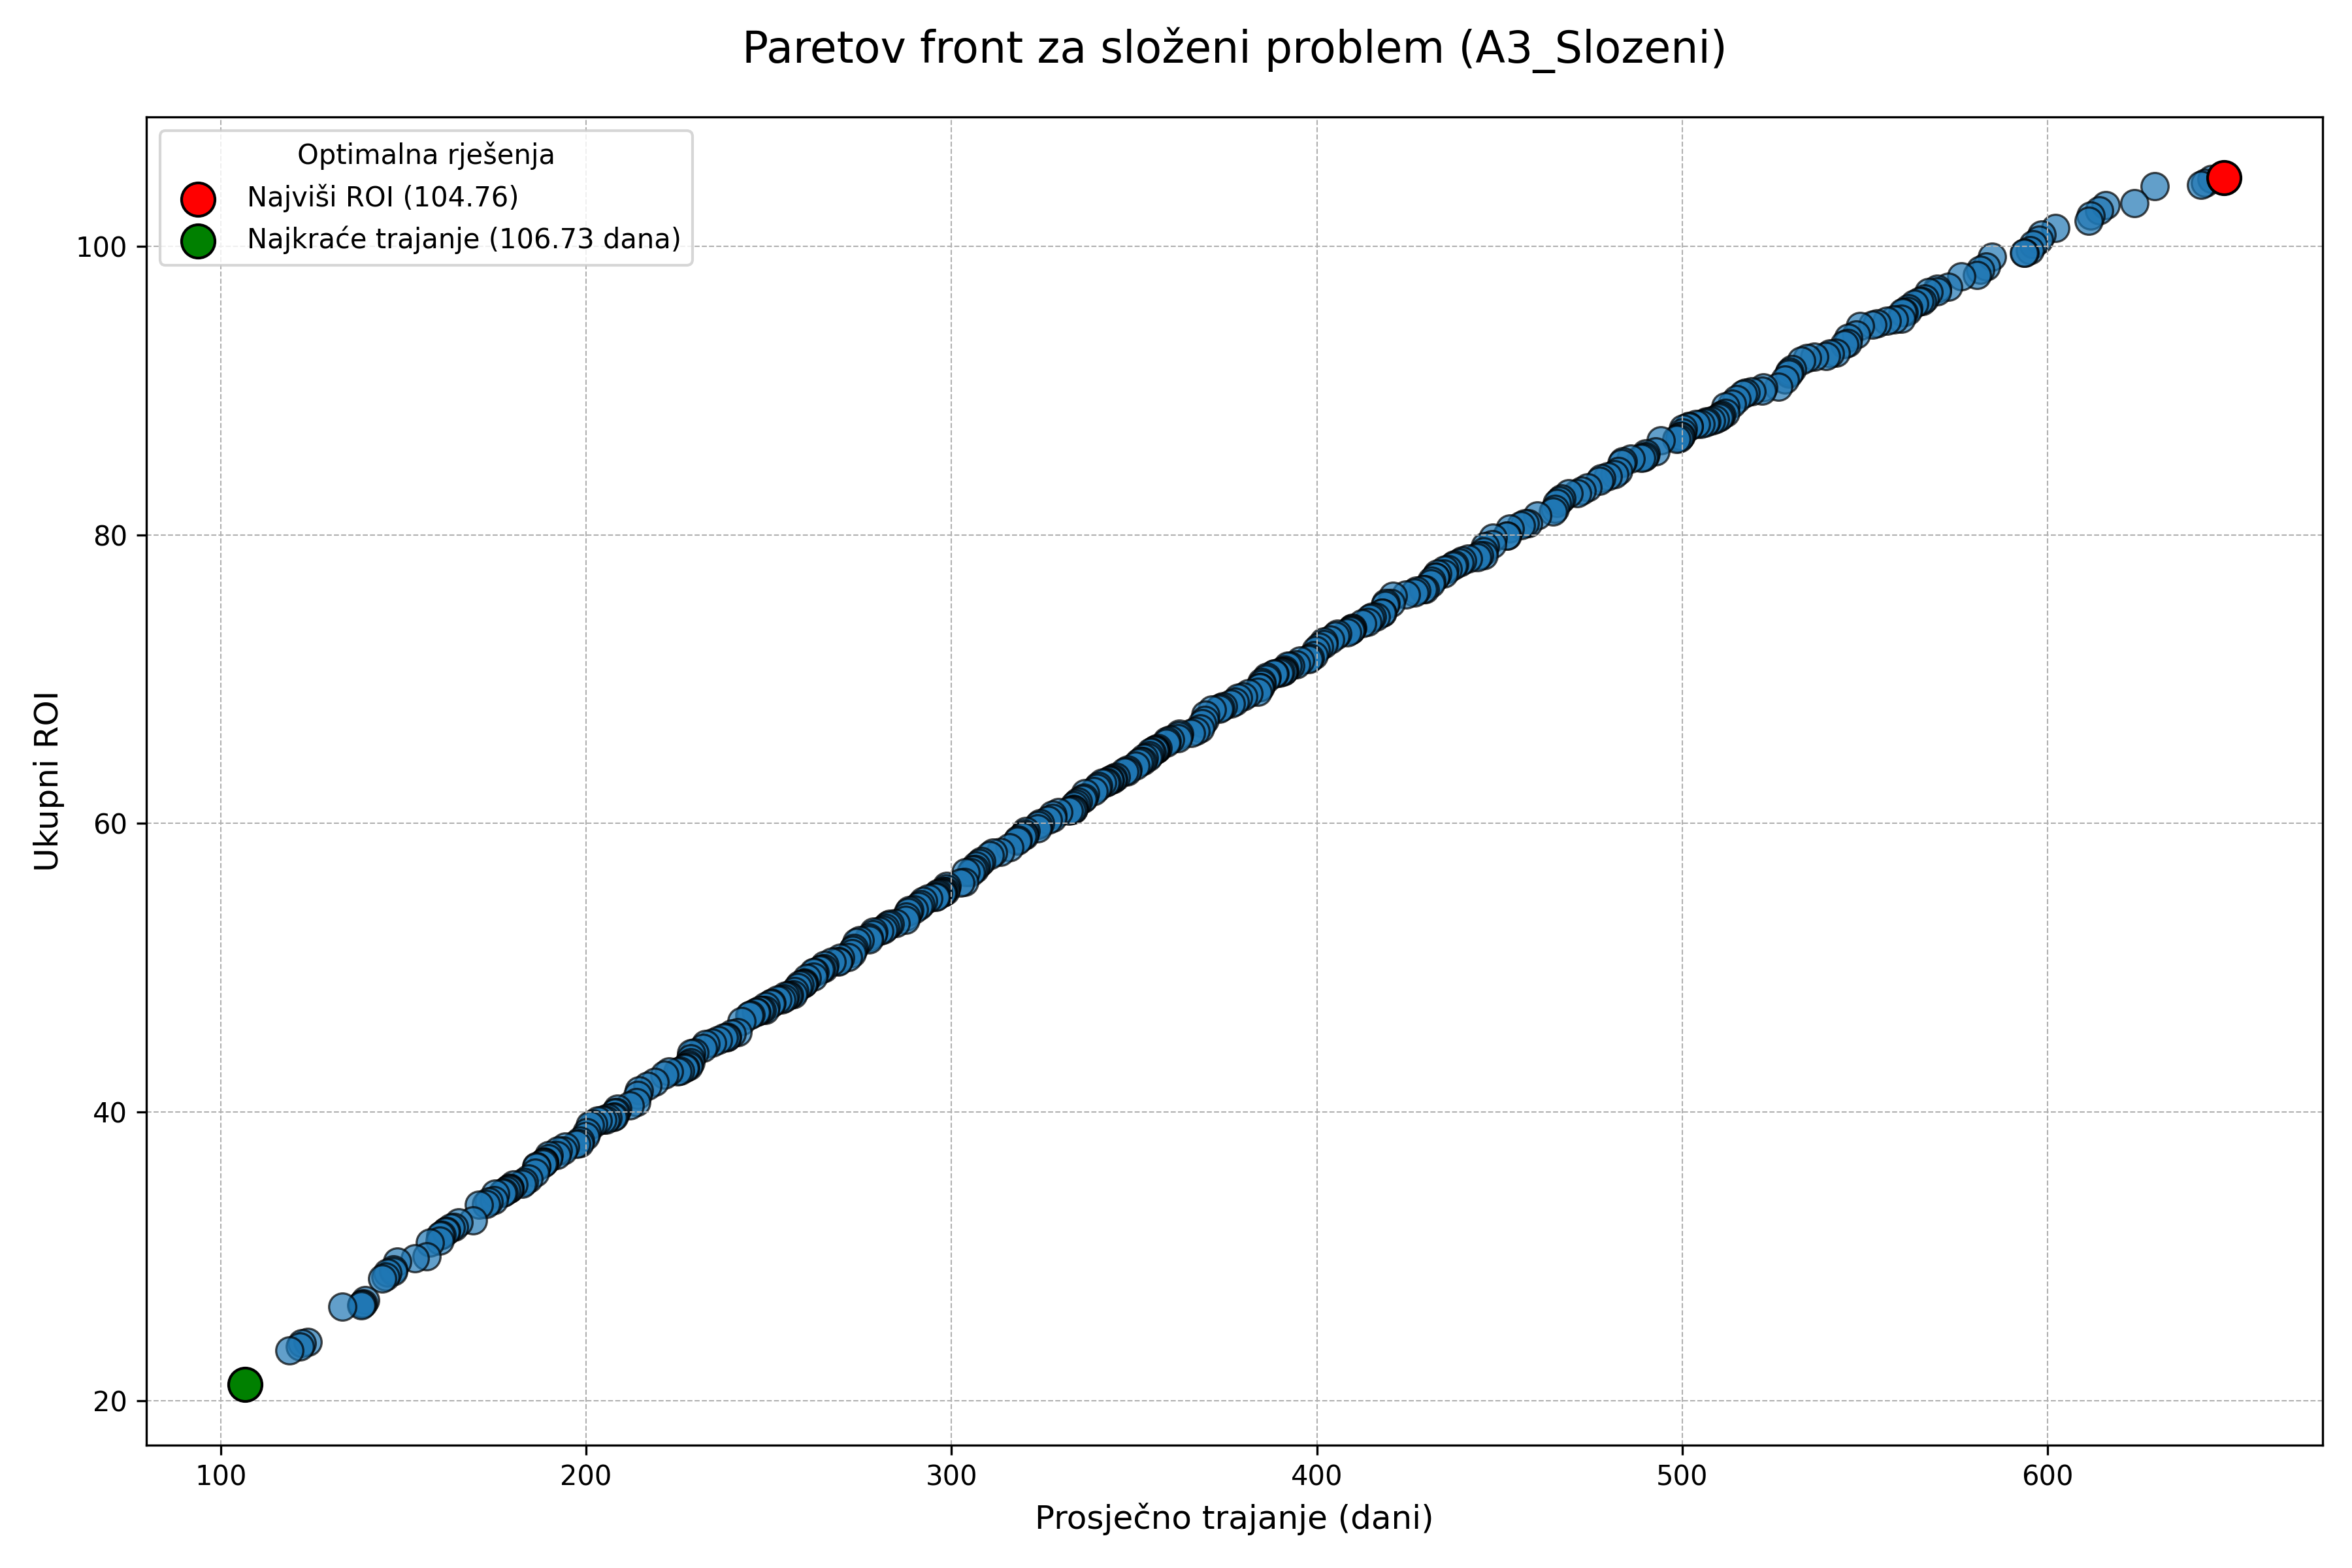
\includegraphics[width=0.9\textwidth]{slike/grafikoni_final/D_pareto_front_scatter.png}
    \caption{Paretov front za složeni problem (A3), koji prikazuje kompromis između ROI-a i trajanja.}
    \label{fig:pareto_front}
\end{figure}

\subsection{Sinteza i interpretacija glavnih nalaza}
Provedeni eksperimenti omogućuju donošenje cjelovitih zaključaka o svakom modelu. Random Search (MC) se pokazao korisnim isključivo kao početna točka na jednostavnim problemima, ali je potpuno neadekvatan kao ozbiljan optimizacijski alat za probleme realne veličine. GA (samo ROI) je izuzetno snažan i robustan "profitni maksimizator", idealan u situacijama gdje je financijska dobit jedini kriterij. Konačno, GA+MC (NSGA-II) je sofisticirani "upravitelj rizikom", čija najveća vrijednost leži u pružanju strateških opcija koje balansiraju profit i rizik. Iako je superioran u standardnim i složenim uvjetima, njegova složenost ga čini osjetljivim u okruženjima s ekstremno restriktivnim ograničenjima.

Konačan izbor modela stoga ovisi o strateškim prioritetima projektnog ureda. Za maksimalan profit, klasični GA je pobjednik. Za uravnoteženo i rizikom informirano donošenje odluka, hibridni GA+MC je superioran, uz nužan oprez pri primjeni u vrlo ograničenim uvjetima.


Nakon detaljne analize pojedinačnih serija eksperimenata, mogu se sintetizirati ključni nalazi koji zajedno oslikavaju cjelovitu sliku o performansama, prednostima i nedostacima svakog od testiranih optimizacijskih modela. Interpretacija ovih nalaza pruža direktne odgovore na postavljene istraživačke hipoteze.

Potvrda superiornosti genetskih algoritama (H1):
Prvi i najjasniji zaključak jest da je hipoteza o skalabilnosti (H1) u potpunosti potvrđena. Iako je Random Search metoda, zbog velikog broja evaluacija, uspijevala pronaći valjana rješenja, njezina učinkovitost nije pratila eksponencijalni rast složenosti problema. S druge strane, oba genetska algoritma pokazala su sposobnost inteligentno vođene pretrage, konzistentno pronalazeći značajno superiornija rješenja. Za projektnog menadžera, praktična implikacija je nedvosmislena: za bilo koji netrivijalan problem odabira portfelja, primjena metaheurističkih metoda poput genetskih algoritama nije samo poboljšanje, već nužnost za postizanje konkurentnih rezultata.

Kvantifikacija kompromisa između profita i rizika (H2):
Središnji nalaz istraživanja proizašao je iz usporedbe dvaju genetskih algoritama. Model GA (samo ROI) se dokazao kao iznimno učinkovit "profitni maksimizator", konzistentno pronalazeći rješenja s najvišim mogućim povratom na investiciju. Međutim, bio je potpuno "slijep" na rizik trajanja, često birajući portfelje s dugim i nepredvidljivim vremenom izvođenja.

Tu do izražaja dolazi ključni doprinos hibridnog GA+MC (NSGA-II) modela. Njegova svrha nije bila nadmašiti klasični GA u jednoj dimenziji (ROI), već otkriti i kvantificirati sam kompromis između profitabilnosti i rizika, čime je potvrđena hipoteza H2. Kao što rezultati i Paretov front (Slika~\ref{fig:pareto_front}) pokazuju, hibridni model omogućuje donošenje strateške odluke. On kvantificira "cijenu" smanjenja rizika, pokazujući, primjerice, da se za 5-10% niži ROI može dobiti portfelj koji je 15-25% brži i, što je još važnije, statistički pouzdaniji. Za donositelja odluka, ovo transformira optimizacijski problem iz potrage za jednim brojem u sofisticirani alat za strateško planiranje.

Otkriće o robusnosti i krhkosti modela (H3):
Konačno, analiza utjecaja ograničenja (Serija B) potvrdila je hipotezu H3 i dovela do najdubljeg i pomalo neočekivanog zaključka. Dok je klasični GA (samo ROI) pokazao iznimnu robusnost, pronalazeći dobra rješenja čak i pod vrlo restriktivnim budžetom, napredni GA+MC (NSGA-II) model pokazao je neočekivanu krhkost. Njegov složeni, više-kriterijski mehanizam pretrage, koji briljira u velikim i otvorenim prostorima rješenja, postao je njegova slabost u ekstremno suženom prostoru valjanih opcija, što je dovelo do čestih neuspjeha.

Ovaj nalaz nosi ključnu praktičnu poruku: tehnološki najnapredniji alat nije uvijek najbolji alat za svaku situaciju. U kriznim scenarijima s ekstremno ograničenim resursima, jednostavniji i fokusiraniji pristup može biti pouzdaniji.

Za lakši pregled, konačna ocjena svakog modela sažeta je u Tablici~\ref{tab:sinteza_modela}.

\begin{table}[H]
\centering
\caption{Sintetička usporedba evaluiranih modela.}
\label{tab:sinteza_modela}
\begin{tabular}{|l|p{4cm}|p{4cm}|}
\hline
\textbf{Model} & \textbf{Najbolji za...} & \textbf{Ključna ograničenja} \\
\hline
\textbf{Random Search (MC)} & Postavljanje osnovne linije (baseline) na jednostavnim problemima. & Potpuno neefikasan i nepouzdan na složenim problemima. \\
\hline
\textbf{GA (samo ROI)} & Scenarije gdje je maksimizacija profita jedini i isključivi cilj. & Zanemaruje rizik trajanja; može predložiti vrlo duge projekte. \\
\hline
\textbf{GA+MC (NSGA-II)} & Strateško odlučivanje; balansiranje između profita i rizika. & Računalno zahtjevan; nepouzdan u ekstremno restriktivnim uvjetima. \\
\hline
\end{tabular}
\end{table}


Konačan izbor modela stoga ovisi o strateškim prioritetima projektnog ureda. Za maksimalan profit, klasični GA je pobjednik. Za uravnoteženo i rizikom informirano donošenje odluka, hibridni GA+MC je superioran, uz nužan oprez pri primjeni u vrlo ograničenim uvjetima.
